\documentclass[12pt]{ociamthesis}  % default square logo 
%\documentclass[12pt,beltcrest]{ociamthesis} % use old belt crest logo
%\documentclass[12pt,shieldcrest]{ociamthesis} % use older shield crest logo

%load any additional packages
\usepackage{amssymb}

%input macros (i.e. write your own macros file called mymacros.tex 
%and uncomment the next line)
%\include{mymacros}

\title{Modul Praktikum \\[1ex]     %your thesis title,
        Kecerdasan Buatan}   %note \\[1ex] is a line break in the title

\author{Rolly Maulana Awangga}             %your name
\college{0410118609\\[5ex]
Applied Bachelor of Informatics Engineering}  %your college

%\renewcommand{\submittedtext}{change the default text here if needed}
\degree{Politeknik Pos Indonesia}     %the degree
\degreedate{Bandung 2019}         %the degree date

%end the preamble and start the document
\begin{document}

%this baselineskip gives sufficient line spacing for an examiner to easily
%markup the thesis with comments
\baselineskip=18pt plus1pt

%set the number of sectioning levels that get number and appear in the contents
\setcounter{secnumdepth}{3}
\setcounter{tocdepth}{3}


\maketitle                  % create a title page from the preamble info
\begin{dedication}
`Jika Kamu tidak dapat menahan lelahnya belajar, \\
Maka kamu harus sanggup menahan perihnya Kebodohan.'\\ 
~Imam Syafi'i~\\
\end{dedication}        % include a dedication.tex file
\begin{acknowledgements}
Pertama-tama kami panjatkan puji dan syukur kepada Allah SWT yang telah memberikan rahmat dan hidayah-Nya sehingga Buku Pedoman Tingkat Akhir ini dapat diselesaikan.
\end{acknowledgements}   % include an acknowledgements.tex file
\begin{abstract}
	Buku Pedoman ini dibuat dengan tujuan memberikan acuan, bagi mahasiswa Tingkat Akhir dan dosen
	Pembimbing. Pada intinya buku ini menjelaskan secara lengkap tentang Standar pengerjaan Intership  dan 
	Tugas Akhir
	di Program Studi D4 Teknik Informatika, dan juga mengatur mekanisme, teknik penulisan, serta
	penilaiannya.Dengan demikian diharapkan semua pihak yang terlibat dalam aktivitas Bimbingan Mahasiswa Tingkat Akhir
	berjalan lancar dan sesuai dengan standar.
\end{abstract}          % include the abstract

\begin{romanpages}          % start roman page numbering
\tableofcontents            % generate and include a table of contents
\listoffigures              % generate and include a list of figures
\end{romanpages}            % end roman page numbering

%now include the files of latex for each of the chapters etc
\chapter{Mengenal Kecerdasan Buatan dan Scikit-Learn}
Buku umum yang digunakan adalah \cite{russell2016artificial} dan  
untuk sebelum UTS menggunakan buku \textit{Python Artificial Intelligence Projects for Beginners}\cite{eckroth2018python}.
Dengan praktek menggunakan python 3 dan editor anaconda dan library python scikit-learn.
Tujuan pembelajaran pada pertemuan pertama antara lain:
\begin{enumerate}
\item
Mengerti definisi kecerdasan buatan, sejarah kecerdasan buatan, perkembangan dan penggunaan di perusahaan
\item
Memahami cara instalasi dan pemakaian sci-kit learn
\item
Memahami cara penggunaan variabel explorer di spyder
\end{enumerate}
Tugas dengan cara dikumpulkan dengan pull request ke github dengan menggunakan latex pada repo yang dibuat oleh asisten riset.

\section{Teori}
Praktek teori penunjang yang dikerjakan :
\begin{enumerate}
\item
Buat Resume Definisi, Sejarah dan perkembangan Kecerdasan Buatan, dengan bahasa yang mudah dipahami dan dimengerti. Buatan sendiri bebas plagiat[hari ke 1](10)
\item
Buat Resume mengenai definisi supervised learning, klasifikasi, regresi dan unsupervised learning. Data set, training set dan testing set.[hari ke 1](10)
\end{enumerate}

\section{Instalasi}
Membuka https://scikit-learn.org/stable/tutorial/basic/tutorial.html. Dengan menggunakan bahasa yang mudah dimengerti dan bebas plagiat. 
Dan wajib skrinsut dari komputer sendiri.
\begin{enumerate}
\item
Instalasi library scikit dari anaconda, mencoba kompilasi dan uji coba ambil contoh kode dan lihat variabel explorer[hari ke 1](10)
\item
Mencoba Loading an example dataset, menjelaskan maksud dari tulisan tersebut dan mengartikan per baris[hari ke 1](10)
\item
Mencoba Learning and predicting, menjelaskan maksud dari tulisan tersebut dan mengartikan per baris[hari ke 2](10)
\item
mencoba Model persistence, menjelaskan maksud dari tulisan tersebut dan mengartikan per baris[hari ke 2](10)
\item 
Mencoba Conventions, menjelaskan maksud dari tulisan tersebut dan mengartikan per baris[hari ke 2](10)
\end{enumerate}


\section{Penanganan Error}
Dari percobaan yang dilakukan di atas, apabila mendapatkan error maka:

\begin{enumerate}
	\item
	skrinsut error[hari ke 2](10)
	\item
Tuliskan kode eror dan jenis errornya [hari ke 2](10)
	\item
Solusi pemecahan masalah error tersebut[hari ke 2](10)

\end{enumerate}


\section{Andri Fajar S/1164065}
\subsection{TEORI}
\begin{enumerate}
\item
Definisi, Sejarah, Dan Perkembangan Sejarah AI
\subitem Didefinisikan  kecerdasan yang ditunjukkan oleh suatu entitas buatan. Umumnya dianggap komputer. Kecerdasan Buatan (Artificial Intelligence atau AI) didefinisikan sebagai kecerdasan yang ditunjukan oleh suatu entitas buatan. Sistem seperti ini umumnnya dianggao kemputer. Kecerdasan dimasukkan ke dalam mesin (komputer) agar dapat melakukan pekerjaan seperti yang dapat dilakukan manusia. Kecerdasan Buatan (Artificial Intelligence atau AI) didefinikasikan sebagai kecerdasan yang ditinjukkan oleh suatu entitas buatan. Sistem seperti ini umumnya di anggap komputer. Kecerdasan diciptakan dan dimasukkan melakukan pekerjaan seperti yang dapat dilakukan manusia. 
\subitem Sejarah dan perkembangan kecerdasan buatan terjadi pada musim panas tahun 1956 tercatat adanya seminar mengenai AI di Darmouth College. Seminar pada waktu itu dihadiri oleh sejumlah pakar komputer dan membahas potensi komputer dalam meniru 
kepandaian manusia. Akan tetapi perkembangan yang sering terjadi semenjak diciptakannya LISP, yaitu bahasa kecerdasan buatan yang dibuat tahun 1960 oleh John McCarthy. Istilah pada kecerdasan buatan atau Artificial Intelligence diambil dari Marvin Minsky dari MIT. Dia menulis karya ilmiah berjudul Step towards Artificial Intelligence,The Institute of radio Engineers Proceedings 49, January 1961\cite{ai2011kecerdasani}.
\subitem Supervised learning merupakan sebuah pendekatan dimana sudah terdapat data yang dilatih, dan terdapat variable yang ditargetkan sehingga tujuan dari pendekatan ini adalah mengkelompokan suatu data ke data yang sudah ada. Sedangkan unsupervised 
learning tidak memiliki data latih, sehingga dari data yang ada, kita mengelompokan data tersebut menjadi 2 bagian atau 3 bagian dan seterusnya.
\subitem Klasifikasi adalah salah satu topik utama dalam data mining atau machine learning. Klasifikasi yaitu suatu pengelompokan data dimana data yang digunakan tersebut mempunyai kelas label atau target.
\subitem Regresi adalah Supervised learning tidak hanya mempelajari classifier, tetapi juga mempelajari fungsi yang dapat memprediksi suatu nilai numerik. Contoh, ketika diberi foto seseorang, kita ingin memprediksi umur, tinggi, dan berat orang yang ada pada foto tersebut.
\subitem Data set adalah cabang aplikasi dari Artificial Intelligence/Kecerdasan Buatan yang fokus pada pengembangan sebuah sistem yang mampu belajar sendiri tanpa harus berulang kali di program oleh manusia.
\item Training set yaitu jika pasangan objek, dan kelas yang menunjuk pada objek tersebut adalah suatu contoh yang telah diberi label akan menghasilkan suatu algoritma pembelajaran.
\subitem Testing set digunakan untuk mengukur sejauh mana classifier berhasil melakukan klasifikasi dengan benar.


\subsection{Instalasi}

\begin{itemize}
\item
Memberikan perintah conda install scikit-learn di cmd, lihat gambar 1.1
\item
Melihat versinya dengan memberikan perintah conda --version dan python --version, lihat gambar 1.2
\item
Install pip, lihat pada gambar 1.3
\item
Hasil Kompile, lihat gambar 1.4
\item
Import dataset kemudian load iris dan data dari digits, lihat gambar 1.5
\item
Melihat data digits
\end{itemize}

\begin{figure}[ht]\centerline{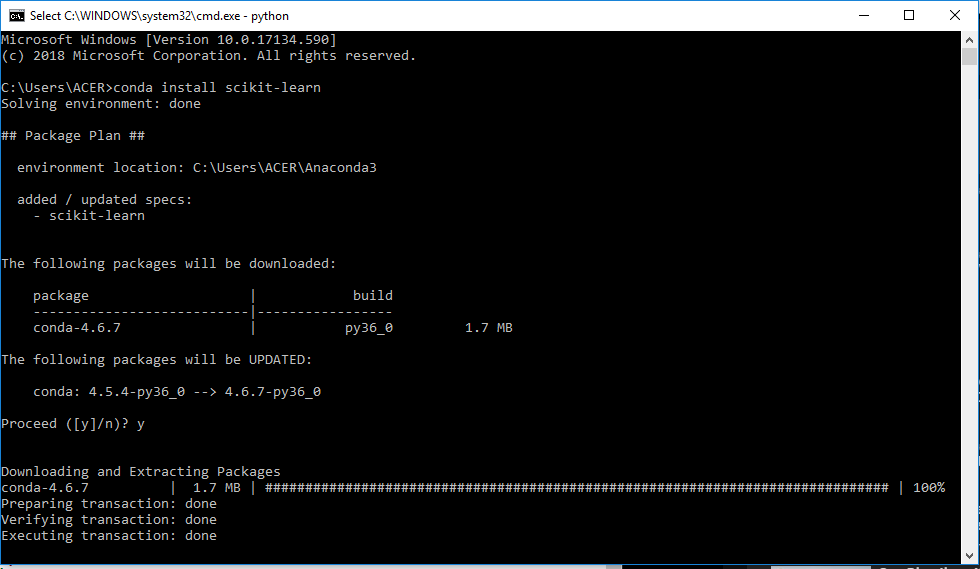
\includegraphics[width=1\textwidth]{figures/111.PNG}}\caption{conda install scikit-learn.}\end{figure}

\begin{figure}[ht]\centerline{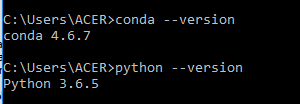
\includegraphics[width=1\textwidth]{figures/222.PNG}}\caption{Melihat Version.}\end{figure}

\begin{figure}[ht]\centerline{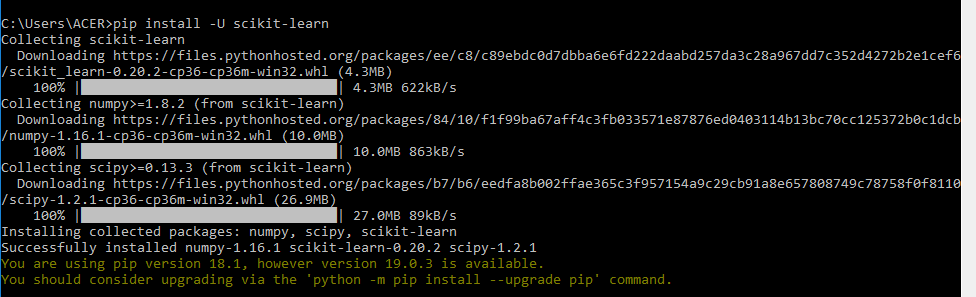
\includegraphics[width=1\textwidth]{figures/333.PNG}}\caption{Install pip.}\end{figure}

\begin{figure}[ht]\centerline{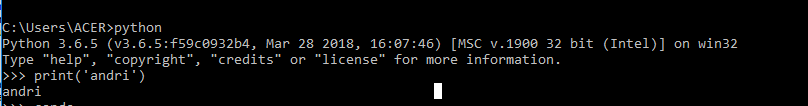
\includegraphics[width=1\textwidth]{figures/444.PNG}}\caption{Hasil Kompile.}\end{figure}

\begin{figure}[ht]\centerline{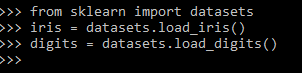
\includegraphics[width=1\textwidth]{figures/555.PNG}}\caption{Hasil Kompile.}\end{figure}

\begin{figure}[ht]\centerline{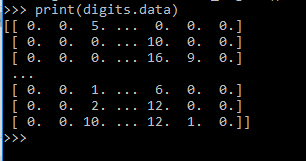
\includegraphics[width=1\textwidth]{figures/666.PNG}}\caption{Hasil Kompile.}\end{figure}
\end{enumerate}



\subsection{Mencoba Learning and predicting}

\begin{enumerate}
\item
Buka CMD lalu ketikan perintah Python.
\begin{figure}
	\begin{center}
   	 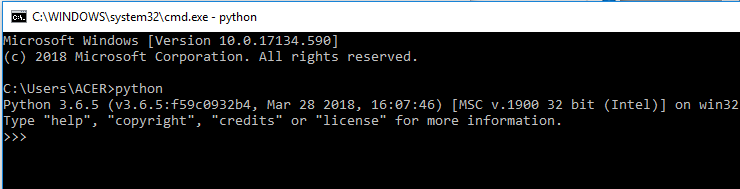
\includegraphics[scale=1]{figures/andri1.png}
   	 \caption{Membuka Python }	
	\end{center}
\end{figure}
\item
 "from sklearn import svm"  artinya akan memanggil dan menggunakan estimator dari kelas sklearn.svm.SVC
\begin{figure}
	\begin{center}
   	 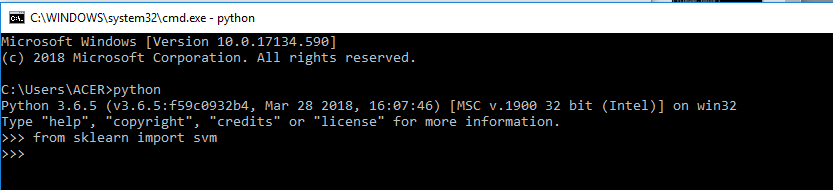
\includegraphics[scale=1]{figures/andri2.png}
   	 \caption{ Estimator Sklearn }	
	\end{center}
\end{figure}
\item
 disini gamma didefinisikan secara manual
\begin{figure}
	\begin{center}
   	 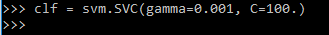
\includegraphics[scale=1]{figures/andri3.png}
   	 \caption{Mendefinisikan Classifier }	
	\end{center}
\end{figure}
\item
Estimator clf (for classifier) pertama kali dipasang pada model. Ini dilakukan dengan melewati training set ke metode fit. Untuk training set, akan menggunakan semua gambar dari set data yang ada, kecuali untuk gambar terakhir, yang dicadangan untuk prediksi. Pada skrip dibawah memilih training set dengan sintaks Python [: -1], yang menghasilkan array baru yang berisi semua kecuali item terakhir dari digits.data
\begin{figure}
	\begin{center}
   	 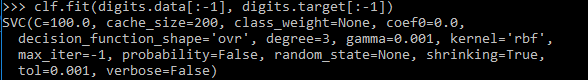
\includegraphics[scale=1]{figures/andri4.png}
   	 \caption{Memanggil Classifier  }	
	\end{center}
\end{figure}
\item
Pada penggalan skrip dibawah, ini menunjukan prediksi nilai baru menggunakan gambar terakhir dari digits.data. 
\begin{figure}
	\begin{center}
   	 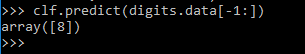
\includegraphics[scale=1]{figures/andri5.png}
   	 \caption{Memprediksi Nilai Baru}	
	\end{center}
\end{figure}
\end{enumerate}

\subsection{Mencoba Model Persistance}
\begin{enumerate}
\item
 "from sklearn import svm" artinya akan mengimport sebuah Support Vector Machine(SVM) yang merupakan algoritma classification yang akan diambil dari Scikit-Learn.
\item
 "from sklearn import datasets"  artinya akan mengambil package datasets dari Scikit-Learn.
\item
ketikan, clf = svm.SVC(gamma='scale') berfungsi untuk mendeklarasikan suatu value yang bernama clf yang berisi gamma.
\item
Ketikan, X, y = iris.data, iris.target, artinya X sebagai data iris, dan y merupakan larik target.
\item
Ketikan, clf.fit(X, y) berfungsi untuk melakukan pengujian classifier. hasilnya seperti ini
\begin{figure}
	\begin{center}
   	 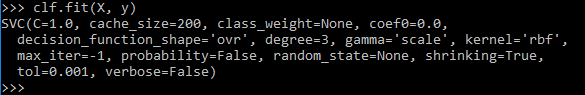
\includegraphics[scale=1]{figures/andri7.png}
   	 \caption{Hasil  Classifier}	
	\end{center}
\end{figure}
\item
\begin{figure}
	\begin{center}
   	 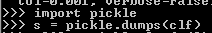
\includegraphics[scale=1]{figures/andri8.png}
   	 \caption{Hasil  Classifier}	
	\end{center}
\end{figure}
Dari gambar diatas dapat dijelaskan bahwa akan mengimport Pickle dari Python. Pickle digunakan untuk serialisasi dan de-serialisasi struktur objek Python. Objek apa pun dengan Python dapat di-Pickle sehingga dapat disimpan di disk. kemudian menyimpan data objek ke file CLF sebelumnya dengan menggunakan function pickle.dumps(clf).
\item
Setelah mengetikan fungsi fungsi diatas, selanjutnya ketikan "clf2 = pickle.loads(s)" yang artinya pickle.loads digunakan untuk memuat data pickle dari string byte. "S" dalam loads mengacu pada fakta bahwa dalam Python 2, data dimuat dari string.
\begin{figure}
	\begin{center}
   	 
\includegraphics[scale=1]{figures/andri9.png}
   	 \caption{Pickle  Python}	
	\end{center}
\end{figure}
\item
\begin{figure}
	\begin{center}
   	 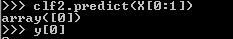
\includegraphics[scale=1]{figures/andri10.png}
   	 \caption{ Classifier Pickle}	
	\end{center}
\end{figure}
Pada gambar diatas dilakukan pengujian nilai baru dengan menggunakan "cf2.predict(X[0:1])" dengan target asumsinya (0,1) hasilnya berbentuk array.
\item
 "from joblib import dump , load" yang artinya akan Merekonstruksi objek Python dari file yang sudah ada.\\

dump(clf, 'filename.joblib') akan merekontruksi file CLF yang tadi sudah dideklarasikan.\\
clf = load('filename.joblib') untuk mereload model yang sudah di Pickle\\
\begin{figure}
	\begin{center}
   	 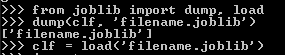
\includegraphics[scale=1]{figures/andri11.png}
   	 \caption{ Joblib}	
	\end{center}
\end{figure}
\end{enumerate}

\subsection{Mencoba Conventions}
\begin{enumerate}
\item
Import numpy as np, digunakan untuk mengimport Numpy sebagai np.\\
From sklearn import randomprojection artinya modul yang mengimplementasikan cara sederhana dan efisien secara komputasi untuk mengurangi dimensi data dengan memperdagangkan sejumlah akurasi yang terkendali (sebagai varian tambahan) untuk waktu pemrosesan yang lebih cepat dan ukuran model yang lebih kecil.
\begin{figure}
	\begin{center}
   	 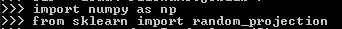
\includegraphics[scale=1]{figures/andri12.png}
   	 \caption{Deklarasi Numpy}	
	\end{center}
\end{figure}
\item
\begin{figure}
	\begin{center}
   	 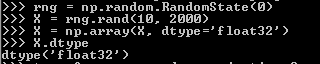
\includegraphics[scale=1]{figures/andri13.png}
   	 \caption{Contoh  Casting}	
	\end{center}
\end{figure}
Pada gambar diatas dapat dijelaskan bahwa :\\
rng = np.random.RandomState(0), digunakan untuk menginisialisasikan random number generator.\\
X = rng.rand(10, 2000) artinya akan merandom value antara 10 sampai 2000.\\
X = np.array(X, dtype='float32') Array numpy terdiri dari buffer memori "mentah" yang diartikan sebagai array melalui "views". Anda dapat menganggap semua array numpy sebagai tampilan. Mendeklarasikan X sebagai float32.
\item
Dalam contoh ini, X adalah float32, yang dilemparkan ke float64 oleh fittransform (X).
\begin{figure}
	\begin{center}
   	 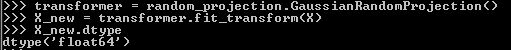
\includegraphics[scale=1]{figures/andri14.png}
   	 \caption{ FitTransform}
	\end{center}
\end{figure}
\item
Target regresi dilemparkan ke float64 dan target klasifikasi dipertahankan.

list(clf.predict(irisdata[:3])), akan memprediksi 3 data dari iris.\\
clf.fit irisdata, iristargetnames[iristarget] menguji classifier dengan ada targetnya yaitu irisnya sendiri.\\
list(clf.predict(irisdata[:3])), setelah diuji maka akan muncul datanya seperti dibawah ini\\
\begin{figure}
	\begin{center}
   	 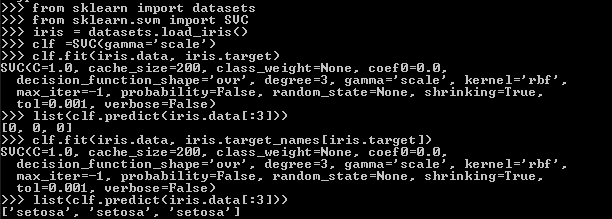
\includegraphics[scale=1]{figures/andri15.png}
   	 \caption{Regresi Yang Dilempar}
	\end{center}
\end{figure}
Di sini, prediksi pertama () mengembalikan array integer, karena iristarget (array integer)yang digunakan sesuai. Prediksi kedua () mengembalikan array string, karena iristargetnames cocok.
\item
Refitting dan Memperbaharui Parameter

y = rngbinomial(1, 0.5, 100) , random value dengan angka binomial atau suku dua untuk y \\
clfsetparams(kernel='linear')fit(X, y) mengubahn kernel default menjadi linear \\
clfsetparams(kernel='rbf', gamma='scale')fit(X, y)  Di sini, kernel default rbf pertama kali diubah menjadi linear melalui\\ SVCsetparams () setelah estimator dibuat, dan diubah kembali ke rbf untuk mereparasi estimator dan membuat prediksi kedua.
\begin{figure}
	\begin{center}
   	 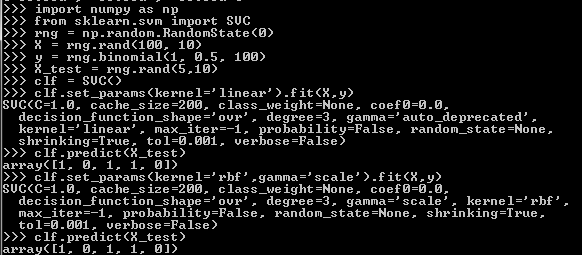
\includegraphics[scale=1]{figures/andri16.png}
   	 \caption{Memperbaharui Parameter}
	\end{center}
\end{figure}
\item
MultiClass VS MultiLabel Classifier \\
from sklearn.multiclass import OneVsRestClassifier ,adalah  ketika kita ingin melakukan klasifikasi multiclass atau multilabel dan baik unutk menggunakan OneVsRestClassifier per kelas. Untuk setiap classifier, kelas tersebut dipasang terhadap semua kelas lainnya. (Ini cukup jelas dan itu berarti bahwa masalah klasifikasi multiclass / multilabel dipecah menjadi beberapa masalah klasifikasi biner).\\
from sklearn.preprocessing import LabelBinarizer ,adalah kelas utilitas untuk membantu membuat matriks indikator label dari daftar label multi-kelas\\
Dalam gambar dibawah, classifier cocok pada array 1d label multiclass dan oleh karena itu metode predict () memberikan prediksi multiclass yang sesuai.
\begin{figure}
	\begin{center}
   	 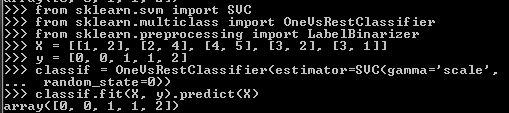
\includegraphics[scale=1]{figures/andri17.png}
   	 \caption{MultiClass }
	\end{center}
\end{figure}
\item
Di sini, classifier cocok () pada representasi label biner 2d dari y, menggunakan LabelBinarizer. Dalam hal ini predict () mengembalikan array 2d yang mewakili prediksi multilabel yang sesuai.
\begin{figure}
	\begin{center}
   	 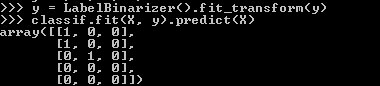
\includegraphics[scale=1]{figures/andri18.png}
   	 \caption{MultiClass  biner 2D}
	\end{center}
\end{figure}
\item
from sklearn.preprocessing import MultiLabelBinarizer , artinya Transformasi antara iterable dari iterables dan format multilabel.\\
Dalam hal ini, penggolongnya sesuai pada setiap instance yang diberi beberapa label. MultiLabelBinarizer digunakan untuk membuat binarize array 2d dari multilabel agar sesuai. Hasilnya, predict () mengembalikan array 2d dengan beberapa label yang diprediksi untuk setiap instance.
\begin{figure}
	\begin{center}
   	 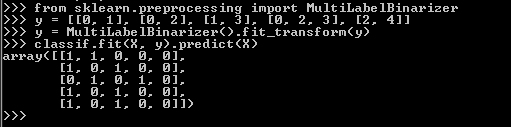
\includegraphics[scale=1]{figures/andri19.png}
   	 \caption{MultiLabel }
	\end{center}
\end{figure}
\end{enumerate}

\section{Penanganan Error}

\begin{enumerate}
	\item
	Berikut ini merupakan eror yang ditemui pada saat melakukan percobaan skrip.
\begin{figure}
	\begin{center}
   	 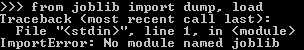
\includegraphics[scale=1]{figures/andrierror.png}
   	 \caption{Eror Import}
	\end{center}
\end{figure}
	\item
Pada gambar eror diatas, kode erornya adalah "ImportError: No Module Named" artinya mengalami masalah saat mengimpor modul yang ditentukan.
	\item
Solusinya bisa dilakukan seperti berikut :\\
eror diats terjadi dikarenakan Library Joblib belum terinstal pada PC. Maka dari itu sekarang kita harus menginstalnya dulu.
	\item
Buka CMD, kemudian ketikan "pip install joblib" tunggu sampai instalasi berhasil seperti gambar berikut.
\begin{figure}
	\begin{center}
   	 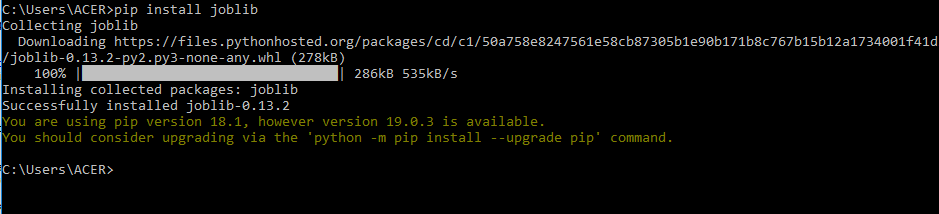
\includegraphics[scale=1]{figures/solusiAndri.png}
   	 \caption{Instal Library Joblib}
	\end{center}
\end{figure}
	\item
Apabila sudah terinstall, dapat dilakukan lagi import library joblib, maka akan berhasil seperti dibawah berikut
\begin{figure}
	\begin{center}
   	 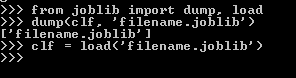
\includegraphics[scale=1]{figures/solusiAndrii.png}
   	 \caption{ Import Library Joblib}
	\end{center}
\end{figure}
\end{enumerate}




\chapter{Related Works}

Your related works, and your purpose and contribution which must be different as below.

\section{Same Topics}
Cite every latest journal with same topic
\subsection{Topic 1}
cite for first topic

\subsection{Topic 2}
if you have two topics you can include here to


\section{Same Method}
write and cite latest journal with same method

\subsection{Method 1}
cite and paraphrase method 1

\subsection{Method 2}
cite and paraphrase method 2 if you have more method please add new subsection.




 \section{Andri Fajar Sunandhar/1164065}
\subsection{binary classification dilengkapi ilustrasi gambar}
\begin{enumerate}
\item Binary classification yaitu berupa kelas positif dan kelas negatif. Klasifikasi biner adalah dikotomisasi yang diterapkan untuk tujuan praktis, dan dalam banyak masalah klasifikasi biner praktis, kedua kelompok tidak simetris - daripada akurasi keseluruhan, proporsi relatif dari berbagai jenis kesalahan yang menarik. Misalnya, dalam pengujian medis, false positive (mendeteksi penyakit ketika tidak ada) dianggap berbeda dari false negative (tidak mendeteksi penyakit ketika hadir).
\begin{figure}[ht]
\centering
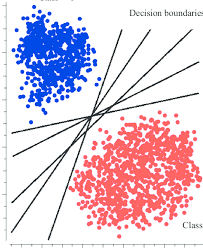
\includegraphics[scale=0.5]{figures/AFS/andri1.png}
\caption{Binary Classification}
\label{contoh}
\end{figure}
\end{enumerate}

\subsection{supervised learning dan unsupervised learning dan clustering dengan ilustrasi gambar}
\begin{enumerate}
\item Supervised learning adalah tugas pembelajaran mesin untuk mempelajari suatu fungsi yang memetakan input ke output berdasarkan contoh pasangan input-output. Ini menyimpulkan fungsi dari data pelatihan berlabel yang terdiri dari serangkaian contoh pelatihan. Dalam pembelajaran yang diawasi, setiap contoh adalah pasangan yang terdiri dari objek input (biasanya vektor) dan nilai output yang diinginkan (juga disebut sinyal pengawas). Algoritma pembelajaran yang diawasi menganalisis data pelatihan dan menghasilkan fungsi yang disimpulkan, yang dapat digunakan untuk memetakan contoh-contoh baru. Skenario optimal akan memungkinkan algoritma menentukan label kelas dengan benar untuk instance yang tidak terlihat. Ini membutuhkan algoritma pembelajaran untuk menggeneralisasi dari data pelatihan untuk situasi yang tidak terlihat dengan cara yang "masuk akal" (lihat bias induktif). Tugas paralel dalam psikologi manusia dan hewan sering disebut sebagai pembelajaran konsep. Contoh dibawah yaitu Supervised Learning dengan SVC.
\begin{figure}[ht]
\centering
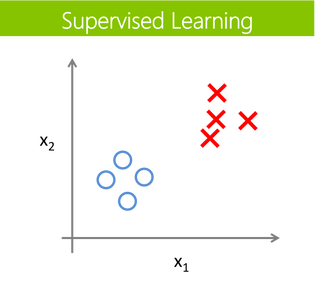
\includegraphics[scale=0.5]{figures/AFS/andri2.png}
\caption{Supervised Learning}
\label{contoh}
\end{figure}
\item Unsupervised learning adalah istilah yang digunakan untuk pembelajaran bahasa Ibrani, yang terkait dengan pembelajaran tanpa guru, juga dikenal sebagai organisasi mandiri dan metode pemodelan kepadatan probabilitas input. Analisis cluster sebagai cabang pembelajaran mesin yang mengelompokkan data yang belum diberi label, diklasifikasikan atau dikategorikan. Alih-alih menanggapi umpan balik, analisis klaster mengidentifikasi kesamaan dalam data dan bereaksi berdasarkan ada tidaknya kesamaan di setiap potongan data baru. BErikut merupakan contoh Unsupervised Learning dengan Gaussian mixture models.
\begin{figure}[ht]
\centering
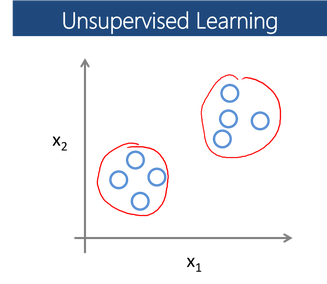
\includegraphics[scale=0.5]{figures/AFS/andri3.png}
\caption{Unsupervised Learning}
\label{contoh}
\end{figure}
\item Cluster analysis or clustering adalah tugas pengelompokan sekumpulan objek sedemikian rupa sehingga objek dalam kelompok yang sama (disebut klaster) lebih mirip (dalam beberapa hal) satu sama lain daripada pada kelompok lain (kluster). Ini adalah tugas utama penambangan data eksplorasi, dan teknik umum untuk analisis data statistik, yang digunakan di banyak bidang, termasuk pembelajaran mesin, pengenalan pola, analisis gambar, pengambilan informasi, bioinformatika, kompresi data, dan grafik komputer. Analisis Cluster sendiri bukan merupakan salah satu algoritma spesifik, tetapi tugas umum yang harus dipecahkan. Ini dapat dicapai dengan berbagai algoritma yang berbeda secara signifikan dalam pemahaman mereka tentang apa yang merupakan sebuah cluster dan bagaimana cara menemukannya secara efisien. Gagasan populer mengenai cluster termasuk kelompok dengan jarak kecil antara anggota cluster, area padat ruang data, interval atau distribusi statistik tertentu. Clustering karena itu dapat dirumuskan sebagai masalah optimasi multi-objektif. Algoritma pengelompokan dan pengaturan parameter yang sesuai (termasuk parameter seperti fungsi jarak yang akan digunakan, ambang kepadatan atau jumlah cluster yang diharapkan) tergantung pada set data individual dan penggunaan hasil yang dimaksudkan. Analisis kluster bukan merupakan tugas otomatis, tetapi proses berulang penemuan pengetahuan atau optimasi multi-objektif interaktif yang melibatkan percobaan dan kegagalan. Seringkali diperlukan untuk memodifikasi praproses data dan parameter model hingga hasilnya mencapai properti yang diinginkan.
\begin{figure}[ht]
\centering
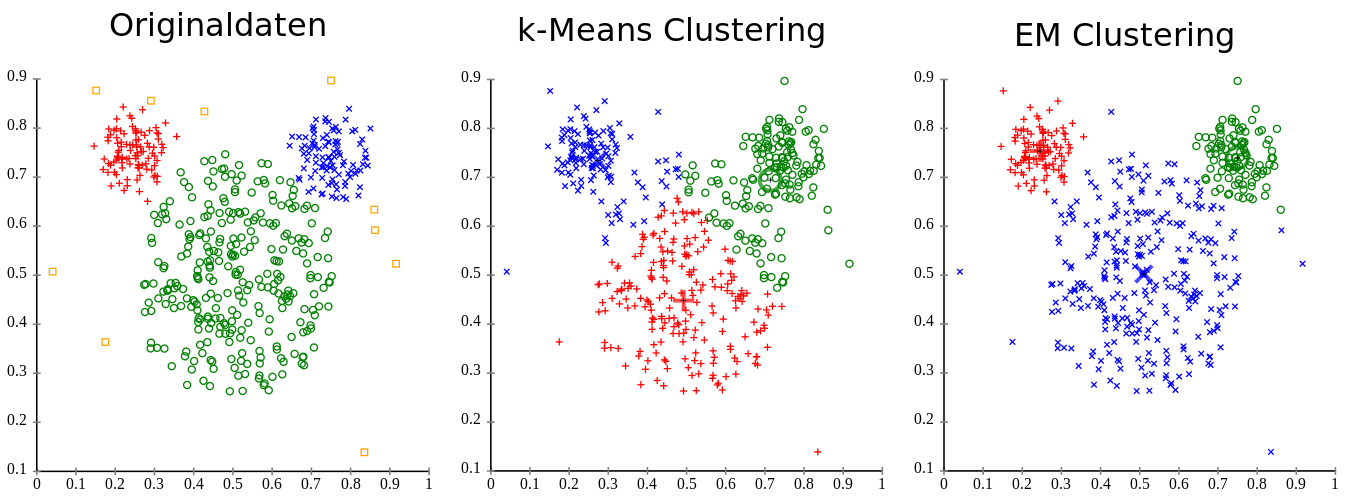
\includegraphics[scale=0.5]{figures/AFS/andri4.png}
\caption{Cluster}
\label{contoh}
\end{figure}
\end{enumerate}

\subsection{evaluasi dan akurasi dari buku dan disertai ilustrasi contoh
dengan gambar}
\begin{enumerate}
\item Evaluasi adalah tentang  bagaimana kita dapat mengevaluasi seberapa baik model bekerja dengan mengukur akurasinya. Dan akurasi akan didefinisikan sebagai persentase kasus yang diklasifikasikan dengan benar. Kita dapat menganalisis kesalahan yang dibuat oleh model, atau tingkat kebingungannya, menggunakan matriks kebingungan. Matriks kebingungan mengacu pada kebingungan dalam model, tetapi matriks kebingungan ini bisa menjadi sedikit sulit untuk dipahami ketika mereka menjadi sangat besar.
\begin{figure}[ht]
\centering
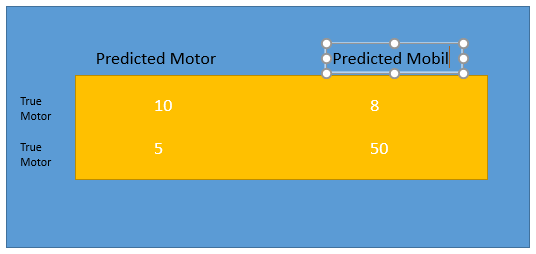
\includegraphics[scale=0.5]{figures/AFS/andri5.png}
\caption{ Evaluasi dan Akurasi}
\label{contoh}
\end{figure}
\end{enumerate}

\subsection{ bagaimana cara membuat dan membaca confusion matrix, buat confusion matrix }
\begin{enumerate}
\item Cara membuat dan membaca confusion matrix :
\begin{itemize}
\item 1)	Tentukan pokok permasalahan dan atributanya, misal gaji dan listik.
\item 2)	Buat pohon keputusan
\item 3)	Lalu data testingnya
\item 4)	Lalu mencari nilai a, b, c, dan d. Semisal a = 5, b = 1, c = 1, dan d = 3.
\item 5)	Selanjutnya mencari nilai recall, precision, accuracy, serta dan error rate.
\end{itemize}
\item Berikut adalah contoh dari confusion matrix :
\begin{itemize}
\item Recall =3/(1+3) = 0,75
\item Precision = 3/(1+3) = 0,75
\item Accuracy =(5+3)/(5+1+1+3) = 0,8
\item Error Rate =(1+1)/(5+1+1+3) = 0,2
\end{itemize}
\end{enumerate}

\subsection{bagaimana K-fold cross validation bekerja dengan gambar ilustrasi}
\begin{enumerate}
\item Cara kerja K-fold cross validation :
\begin{itemize}
\item 1)	Total instance dibagi menjadi N bagian.
\item 2)	Fold yang pertama adalah bagian pertama menjadi data uji (testing data) dan sisanya menjadi training data.
\item 3)	Lalu hitung akurasi berdasarkan porsi data tersebut dengan menggunakan persamaan.
\item 4)	Fold yang ke dua adalah bagian ke dua menjadi data uji (testing data) dan sisanya training data. 
\item 5)	Kemudian hitung akurasi berdasarkan porsi data tersebut.
\item 6)	Dan seterusnya hingga habis mencapai fold ke-K.
\item 7)	Terakhir hitung rata-rata akurasi K buah.
\end{itemize}
\begin{figure}[ht]
\centering
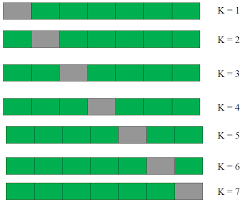
\includegraphics[scale=0.5]{figures/AFS/andri6.png}
\caption{K-fold cross validation }
\label{contoh}
\end{figure}
\end{enumerate}

\subsection{decision tree dengan gambar ilustrasi}
\begin{enumerate}
\item Decision Tree dalah metode pembelajaran yang diawasi non-parametrik yang digunakan untuk klasifikasi dan regresi. Tujuannya adalah untuk membuat model yang memprediksi nilai variabel target dengan mempelajari aturan keputusan sederhana yang disimpulkan dari fitur data.\\
Misalnya, dalam contoh di bawah ini, decision tree belajar dari data untuk memperkirakan kurva sinus dengan seperangkat aturan keputusan if-then-else. Semakin dalam pohon, semakin rumit aturan keputusan dan semakin bugar modelnya.
\begin{figure}[ht]
\centering
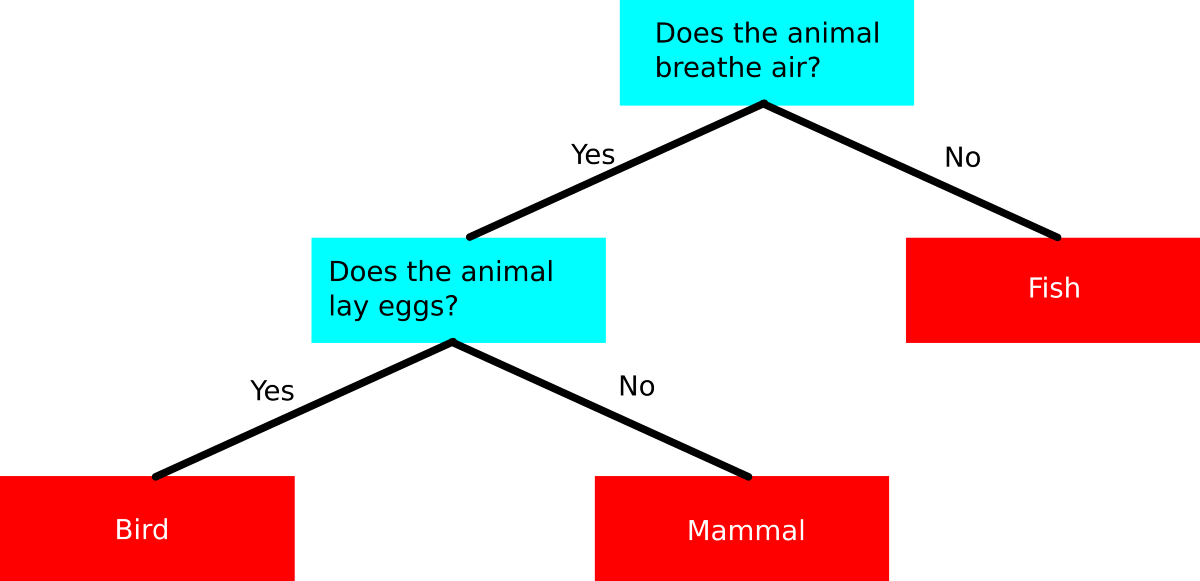
\includegraphics[scale=0.5]{figures/AFS/andri7.png}
\caption{Decision Tree}
\label{contoh}
\end{figure}
\end{enumerate}

\subsection{Information Gain dan entropi dengan gambar ilustrasi}
\begin{enumerate}
\item Information gain didasarkan pada penurunan entropi setelah dataset dibagi pada atribut. Membangun decision tree adalah semua tentang menemukan atribut yang mengembalikan perolehan informasi tertinggi (mis., Cabang yang paling homogen).
\begin{figure}[ht]
\centering

\includegraphics[scale=0.5]{figures/AFS/andri8.png}
\caption{Information gain}
\label{contoh}
\end{figure}
\item Entropi adalah ukuran keacakan dalam informasi yang sedang diproses. Semakin tinggi entropi, semakin sulit untuk menarik kesimpulan dari informasi itu. Membalik koin adalah contoh tindakan yang memberikan informasi yang acak. Untuk koin yang tidak memiliki afinitas untuk kepala atau ekor, hasil dari sejumlah lemparan sulit diprediksi. Mengapa? Karena tidak ada hubungan antara membalik dan hasilnya. Inilah inti dari entropi.
\end{enumerate}

\section{scikit-learn}
HARI KEDUA ANDRI FAJAR SUNANDHAR 1164065

\begin{enumerate}

\item
\begin{verbatim}
	# load dataset (student Portuguese scores)
	import pandas as apel
	jeruk = apel.read_csv('E:\KAMPUS\Semester 6\Kecerdasan Buatan\modul\Python-Artificial-Intelligence-Projects-for-			 	Beginners\Chapter01\dataset\student-mat.csv', sep=';')
	len(jeruk)
\end{verbatim}

\par
Untuk mengimport atau memanggil module pandas sebagai apel. Kemudian mendefinisikan variabel "jeruk" yang akan memanggil dataset yang didapatkan dari data student-mat.csv 
\begin{figure}[ht]
\centering
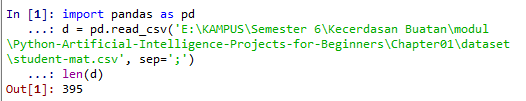
\includegraphics[scale=0.5]{figures/spyder/1.png}
\caption{Loading Dataset}
\label{Spyder}
\end{figure}
\item
\begin{verbatim}
	# generate binary label (pass/fail) based on G1+G2+G3 (test grades, each 0-20 pts); threshold for passing is sum>=30
	jeruk['pass'] = jeruk.apply(lambda row: 1 if (row['G1']+row['G2']+row['G3']) >= 35 else 0, axis=1)
	jeruk = jeruk.drop(['G1', 'G2', 'G3'], axis=1)
	jeruk.head()
\end{verbatim}

\par
mendeklarasikan label pass/fail nya data berdasarkan G1+G2+G3. 
kemudian pada variabel jeruk dideklarasikan  jika baris dengan G1+G2+G3 ditambahkan, dan hasilnya sama dengan 35 maka axisnya 1. 
\begin{figure}[ht]
\centering
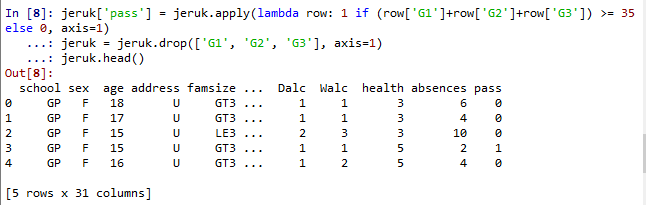
\includegraphics[scale=0.5]{figures/spyder/2.png}
\caption{Generate Binary Label}
\label{Spyder}
\end{figure}
\item
\begin{verbatim}
	# use one-hot encoding on categorical columns
	jeruk = apel.get_dummies(jeruk, columns=['sex', 'school', 'address', 'famsize', 'Pstatus', 'Mjob', 'Fjob', 
                               'reason', 'guardian', 'schoolsup', 'famsup', 'paid', 'activities',
                               'nursery', 'higher', 'internet', 'romantic'])
	jeruk.head()
\end{verbatim}
\par
One-hot encoding adalah proses di mana variabel kategorikal dikonversi menjadi bentuk yang dapat disediakan untuk algoritma .
\begin{figure}[ht]
\centering
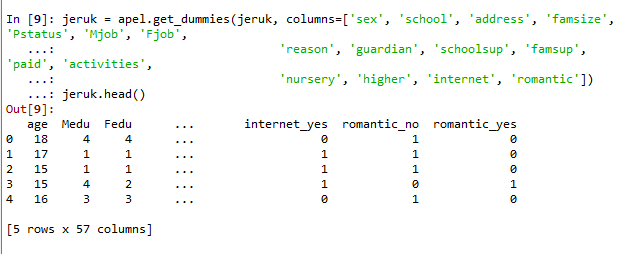
\includegraphics[scale=0.5]{figures/spyder/3.png}
\caption{One-hot Encoding}
\label{Spyder}
\end{figure}
\item
\begin{verbatim}
	# shuffle rows
	jeruk = jeruk.sample(frac=1)
	# split training and testing data
	jeruk_train = jeruk[:500]
	jeruk_test = jeruk[500:]

	jeruk_train_att = jeruk_train.drop(['pass'], axis=1)
	jeruk_train_pass = jeruk_train['pass']

	jeruk_test_att = jeruk_test.drop(['pass'], axis=1)
	jeruk_test_pass = jeruk_test['pass']

	jeruk_att = jeruk.drop(['pass'], axis=1)
	jeruk_pass = jeruk['pass']

	# number of passing students in whole dataset:
	import numpy as np
	print("Passing: %d out of %d (%.2f%%)" % (np.sum(jeruk_pass), len(jeruk_pass), 100*float(np.sum(jeruk_pass)) / 	len(jeruk_pass)))
\end{verbatim}

\par
 Pada bagian tersebut, terdapat train dan test yaing digunakan untuk untuk membagi train, test dan kemudian membagi lagi train ke validasi dan test.\\
Kemudia akan mengimport module numpy sebagai np yang akan digunakan untuk mengembalikan nilai passing dari pelajar dari keseluruhan dataset dengan cara print.
\begin{figure}[ht]
\centering
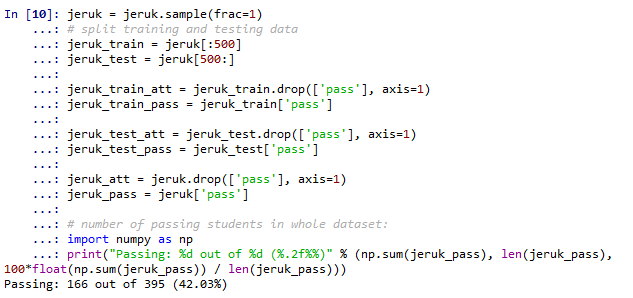
\includegraphics[scale=0.5]{figures/spyder/4.png}
\caption{Shuffle Rows}
\label{Spyder}
\end{figure}
\item 
\begin{verbatim}
	# fit a decision tree
	from sklearn import tree
	semangka = tree.DecisionTreeClassifier(criterion="entropy", max_depth=5)
	semangka = semangka.fit(jeruk_train_att, jeruk_train_pass)
\end{verbatim}

\par
Dari librari scikitlearn import modul tree. Kemudian definisikan variabel semangka dengan menggunakan DecisionTreeClassifier. Kemudian pada variabel semangka terdapat Criterion , setelah itu agar DecisionTreeClassifier dapat dijalankan gunakan perintah fit. hasilnya seperti dibawah
\begin{figure}[ht]
\centering
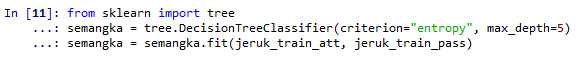
\includegraphics[scale=0.5]{figures/spyder/5.png}
\caption{Fit Decision Tree}
\label{Spyder}
\end{figure}
\item
\begin{verbatim}
	# visualize tree
	import graphviz
	dot_data = tree.export_graphviz(semangka, out_file=None, label="all", impurity=False, proportion=True,
                                feature_names=list(jeruk_train_att), class_names=["fail", "pass"], 
                                filled=True, rounded=True)
	graph = graphviz.Source(dot_data)
	graph
\end{verbatim}

\par
Mengimport Graphviz Sehingga akan muncul gambardiagram  grafik bercabang.
\begin{figure}[ht]
\centering
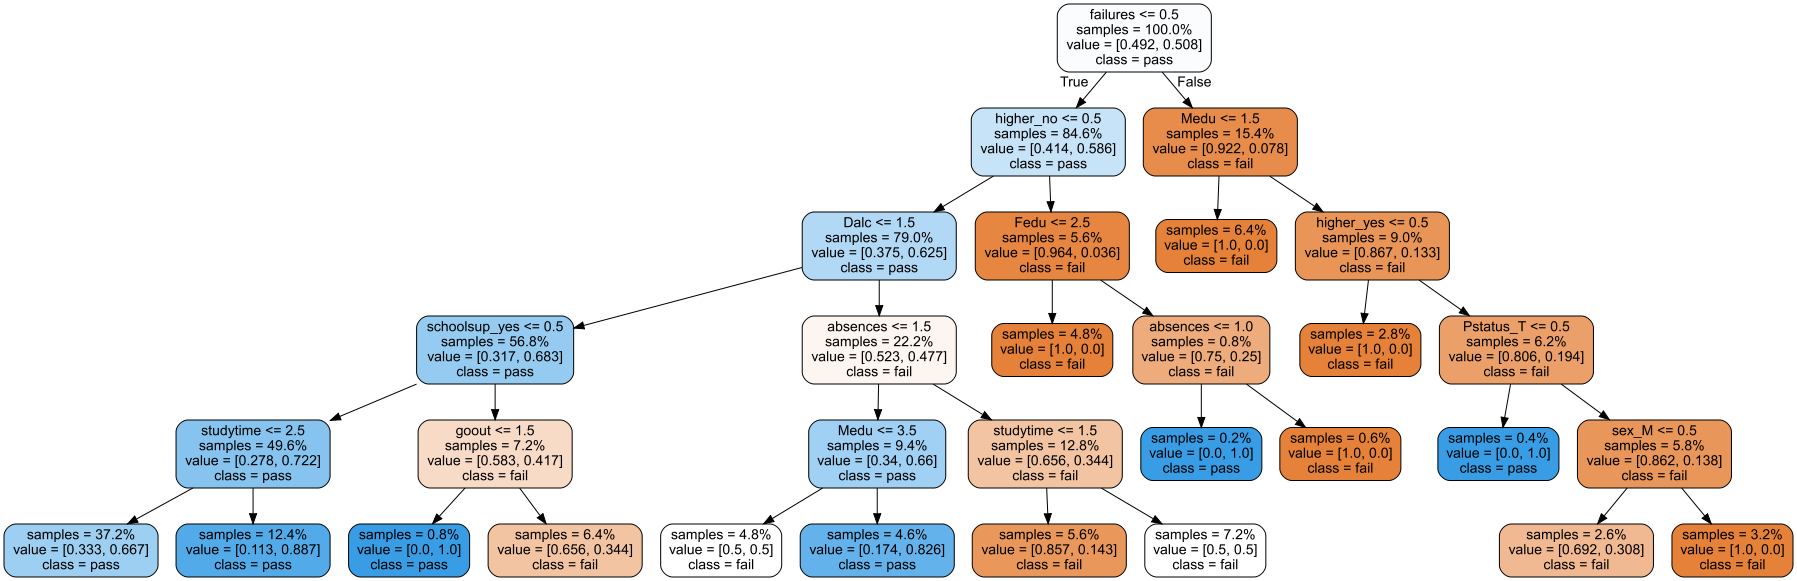
\includegraphics[scale=0.5]{figures/spyder/6.png}
\caption{Fit Decision Tree}
\label{Spyder}
\end{figure}
\item
\begin{verbatim}
	# save tree
	tree.export_graphviz(semangka, out_file="student-performance.dot", label="all", impurity=False, proportion=True,
                     feature_names=list(jeruk_train_att), class_names=["fail", "pass"], 
                     filled=True, rounded=True)
\end{verbatim}

\par
tree.exportgraphviz merupakan fungsi yang menghasilkan representasi Graphviz dari decision tree.
\begin{figure}[ht]
\centering
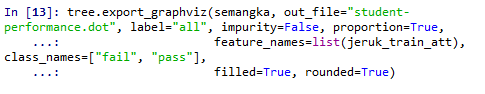
\includegraphics[scale=0.5]{figures/spyder/7.png}
\caption{Fit Decision Tree}
\label{Spyder}
\end{figure}
\item
\begin{verbatim}
	semangka.score(jeruk_test_att, jeruk_test_pass)
\end{verbatim}

\par
Score juga disebut prediksi, Nilai atau skor yang dibuat dapat mewakili prediksi nilai masa depan, tetapi mereka juga mungkin mewakili kategori atau hasil yang mungkin. disini semangka akan memprediksi jeruk.
\begin{figure}[ht]
\centering
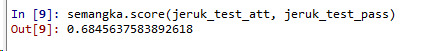
\includegraphics[scale=0.5]{figures/spyder/88.jpeg}
\caption{Score}
\label{Spyder}
\end{figure}
\item
\begin{verbatim}
	from sklearn.model_selection import cross_val_score
	scores = cross_val_score(semangka, jeruk_att, jeruk_pass, cv=5)
	# show average score and +/- two standard deviations away (covering 95% of scores)
	print("Accuracy: %0.2f (+/- %0.2f)" % (scores.mean(), scores.std() * 2))
\end{verbatim}

\par
 Dari sklearn.modelselection akan mengimport crossvalscore. Kemudian akan menampilkan score rata rata dan kurang lebih dua standar deviasi yang mencakup 95 persen score.
\begin{figure}[ht]
\centering
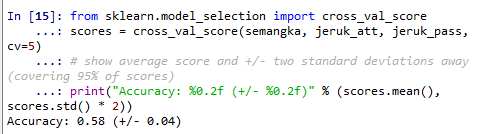
\includegraphics[scale=0.5]{figures/spyder/9.png}
\caption{Cross Val Score}
\label{Spyder}
\end{figure}
\item 
\begin{verbatim}
	for max_depth in range(1, 20):
   	 semangka = tree.DecisionTreeClassifier(criterion="entropy", max_depth=max_depth)
    	scores = cross_val_score(semangka, jeruk_att, jeruk_pass, cv=5)
    	print("Max depth: %d, Accuracy: %0.2f (+/- %0.2f)" % (max_depth, scores.mean(), scores.std() * 2))
\end{verbatim}

\par
Semangka akan mendefinisikan tree.DecissionTreeClassifier nya yang kemudian variabel semangka akan mengevaluasi score dengan validasi silang.
\begin{figure}[ht]
\centering
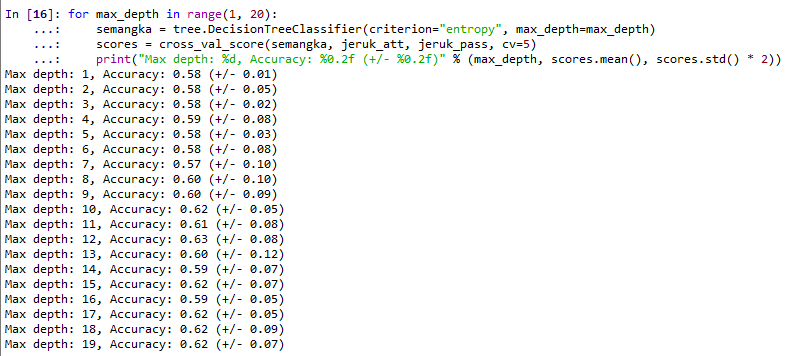
\includegraphics[scale=0.5]{figures/spyder/10.png}
\caption{Max Depth}
\label{Spyder}
\end{figure}
\item
\begin{verbatim}
	depth_acc = np.empty((19,3), float)
	i = 0
	for max_depth in range(1, 20):
    	semangka = tree.DecisionTreeClassifier(criterion="entropy", max_depth=max_depth)
    	scores = cross_val_score(semangka, jeruk_att, jeruk_pass, cv=5)
   	 depth_acc[i,0] = max_depth
   	 depth_acc[i,1] = scores.mean()
   	 depth_acc[i,2] = scores.std() * 2
   	 i += 1
    
	depth_acc

\end{verbatim}

\par
Dengan 19 sebagai bentuk array kosong, 3 sebagai output data-type dan float urutan kolom-utama (gaya Fortran) dalam memori. variabel semangka yang akan melakukan split score dan nangka akan mengvalidasi score secara silang. 
\begin{figure}[ht]
\centering
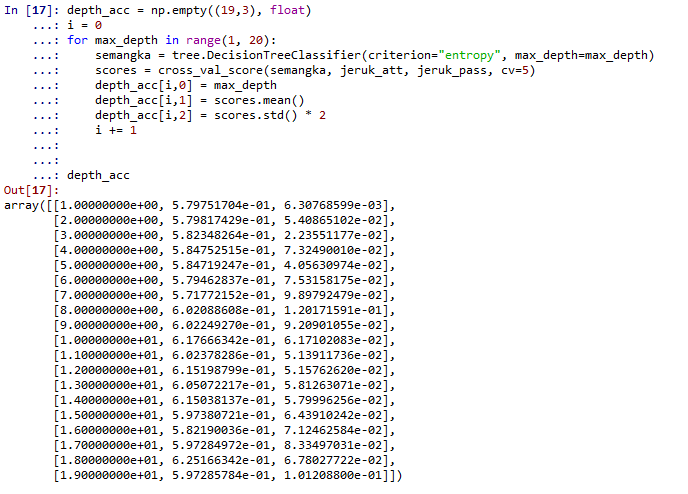
\includegraphics[scale=0.5]{figures/spyder/11.png}
\caption{Depth in Range}
\label{Spyder}
\end{figure}
\item 
\begin{verbatim}
	import matplotlib.pyplot as plt
	fig, ax = plt.subplots()
	ax.errorbar(depth_acc[:,0], depth_acc[:,1], yerr=depth_acc[:,2])
	plt.show()
\end{verbatim}

\par
Mengimpor librari dari matplotlib yaitu pylot sebagai plt\\
fig dan ax menggunakan subplots untuk membuat gambar .\\
ax.errorbar akan membuat error bar
\\
\\
\\
\begin{figure}[ht]
\centering
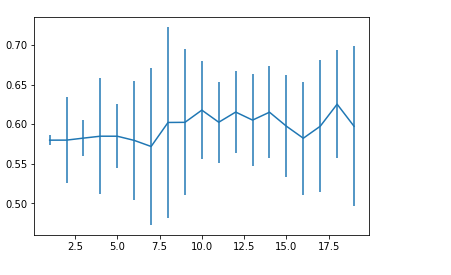
\includegraphics[scale=0.5]{figures/spyder/12.png}
\caption{Matplotlib}
\label{Spyder}
\end{figure}
\end{enumerate}

\section{Penanganan Error}
Hari Kedua Andri fajar Sunandhar 1164065
\subsection{Error Graphviz}
\begin{enumerate}
	\item
error yang didapatkan saat menjalankan Graphviz
\begin{figure}[ht]
\centering
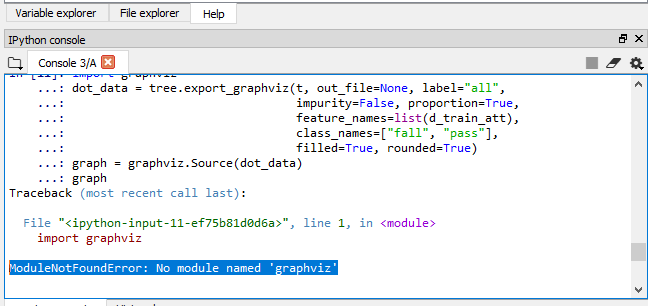
\includegraphics[scale=0.5]{figures/spyder/20.png}
\caption{Error Graphviz}
\label{Error}
\end{figure}
	\item
Kode erornya adalah ModuleNotFoundError. Eror ini terjadi karena module named Graphviz nya tidak ada.
	\item
Solusi yang bisa dilakukan untuk mengatasi eror tersebut adalah sebagai berikut : \\
\begin{itemize}
\item
buka CMD kemudian perintah pip install graphviz
\begin{figure}[ht]
\centering
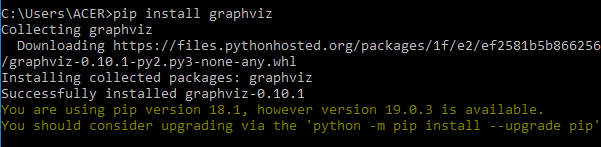
\includegraphics[scale=0.5]{figures/spyder/21.png}
\caption{install Graphviz}
\label{solusi}
\end{figure}
\item
masukan perintah conda install pip, untuk solving environment
\begin{figure}[ht]
\centering
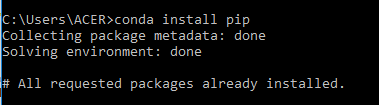
\includegraphics[scale=0.5]{figures/spyder/22.png}
\caption{Solving Environment}
\label{solusi}
\end{figure}
\item
selanjutnya masukan perintah conda install python-graphviz , untuk menambahkan package python-graphviz pada conda
\begin{figure}[ht]
\centering
\includegraphics[scale=0.5]{figures/spyder/23.png}
\caption{Evaluasi Eror}
\label{Eror}
\end{figure}
\end{itemize}
\end{enumerate}


\chapter{Methods}
\extrafloats{100}
\maxdeadcycles=200

\section{The data}
PLease tell where is the data come from, a little brief of company can be put here.

\section{Method 1}
Definition, steps, algoritm or equation of method 1 and how to apply into your data
\section{Method 2}
Definition, steps, algoritm or equation of method 2 and how to apply into your data

\section{Andri Fajar Sunandhar/1164065}
\subsection{Teori}
\begin{enumerate}
\item Apa itu Random Forest Serta Gambar Ilustrasinya \par
Random Forest adalah suatu algoritma yang digunakan pada klasifikasi data dalam jumlah yang besar. Klasifikasi random forest dilakukan melalui penggabungan pohon  dengan melakukan training pada sampel data yang dimiliki. Penggunaan tree yang semakin banyak akan mempengaruhi akurasi yang akan didapatkan menjadi lebih baik. Penentuan klasifikasi dengan random forest diambil berdasarkan hasil voting dari pohon yang terbentuk. Pemenang dari pohon yang terbentuk ditentukan dengan vote terbanyak. Pembangunan pohon  pada random forest sampai dengan mencapai ukuran maksimum dari pohon data. Akan tetapi, pembangunan pohon Random Forest tidak dilakukan pemangkasan  yang merupakan sebuah metode untuk mengurangi kompleksitas ruang. Contoh Ilustrasi sederhana Gambar Random Forest. 
		\begin{figure}[ht]
		\centerline{\includegraphics[width=1\textwidth]{figures/AFS/AFS1.png}}
		\caption{Random Forest.}
		\label{AFS1}
		\end{figure}

\item Cara Membaca Dataset
	

		\begin{enumerate}
			\item Buka Anaconda Navigator.
			\item Jalankan Spyder
			\item Import libraries yang dibutuhkan
			\item Masukan kode berikut untuk membaca file Data.csv.
				\begin{figure}[ht]
				\centering
				\includegraphics[scale=0.8]{figures/AFS/2.png}
				\caption{Kode membaca file.csv}
				\label{contoh}
				\end{figure}
			\item Jalankan kode tersebut, maka di windiws console akan muncul pesan :
				\begin{figure}[ht]
				\centering
				\includegraphics[scale=0.9]{figures/AFS/3.png}
				\caption{ Window Console}
				\label{contoh}
				\end{figure}
			\item Klik variable explorer, maka akan terlihat dataset yang baru ter-import.
				\begin{figure}[ht]
				\centering
				\includegraphics[scale=0.6]{figures/AFS/4.png}
				\caption{Variable Explorer}
				\label{contoh}
				\end{figure}
			\item Kemudian double klik pada dataset cell, maka akan muncul pop-up windows seperti berikut: 
				\begin{figure}[ht]
				\centering
				\includegraphics[scale=0.7]{figures/AFS/5.png}
				\caption{ Dataset Cell}
				\label{contoh}
				\end{figure}
			\item Seperti yang terlihat pada gambar tersebut dataset ini memiliki Kolom Country, Age, dan Salary sebagai 		   				independent variable-nya dan kolom Purchased sebagai dependent variable-nya.			
		\end{enumerate}
	

\item Cross Validation \par
Cross validation adalah metode statistik yang digunakan untuk memperkirakan keterampilan model pembelajaran mesin. Ini biasanya digunakan dalam pembelajaran mesin yang diterapkan untuk membandingkan dan memilih model untuk masalah pemodelan prediktif yang diberikan karena mudah dipahami, mudah diimplementasikan, dan menghasilkan estimasi keterampilan yang umumnya memiliki bias lebih rendah daripada metode lainnya.

\item Arti Score 44\% Pada Random Forest, 27\% Pada Decision Tree dan 29\% Dari SVM \par
\begin{enumerate}
\item Arti Score 44\% \par
Pada Random Forest, Score tersebut merupakan hasil dari akurasi.
\item Arti Score 27\% \par
Pada decission tree adalah presentasi hasil dari perhitungan dataset.
\item Arti Score 29\% Pada SVM \par
merupakan hasil pendekatan jaringan saraf. Jaringan saraf sendiri merupakan komponen jaringan utama dari sistem saraf. Sistem tersebut mengatur dan mengontrol fungsi tubuh dan aktivitas dan terdiri dari dua bagian:  (SSP) yang terdiri dari otak dan sumsum tulang belakang, dan percabangan saraf perifer dari sistem saraf tepi (SST) yang terdapat dalam pengolahan dataset terkait. 
\end{enumerate}

\begin {enumerate}
\item Confusion Matrix Dan Ilustrasinya
\end{enumerate}

\begin{enumerate}
\item Perhitungan confusion matrix adalah sebagai berikut, akan saya beri contoh sederhana yaitu pengambilan keputusan untuk mendapatkan bantuan beasiswa. Saya menggunakan dua atribut, yaitu rekening listrik dan gaji. Ini adalah pohon keputusannya:
 
\begin{figure}[ht]
\centering
\includegraphics[scale=0.5]{figures/AFS/7.jpg}
\caption{Pohon Keputusan}
\label{contoh}
\end{figure}

\end{enumerate}


Kemudian data testingnya adalah

\begin{figure}[ht]
\centering
\includegraphics[scale=0.5]{figures/AFS/8.jpg}
\caption{Data Testing}
\label{contoh}
\end{figure}

Yang pertama kita lakukan yaitu mencari 4 nilai yaitu a,b,c, dan d:

 a= 5

 b= 1

 c= 1

 d= 3

Kemudian kita dapat mencari nilai Recall, Precision, accuracy dan Error Rate

 Recall =3/(1+3) = 0,75

 Precision = 3/(1+3) = 0,75

 Accuracy =(5+3)/(5+1+1+3) = 0,8

 Error Rate =(1+1)/(5+1+1+3) = 0,2

\item Jelaskan Voting Pada Random Forest Beserta Ilustrasinya 
\par Voting merupakan metode yang paling umum digunakan dalam random forest. Ketika classifier membuat keputusan, Anda dapat memanfaatkan yang terbaik keputusan umum dan rata-rata yang didefinisikan ke dalam bentuk "voting".
\par Setelah pohon terbentuk,maka akan dilakukan voting pada setiap kelas dari data sampel. Kemudian, mengkombinasikan vote dari setiap kelas kemudian diambil vote yang paling banyak.Dengan menggunakan random forest pada klasifikasi data maka, akan menghasilkan vote yang paling baik. \ref{AFS6}
		\begin{figure}[ht]
		\centerline{\includegraphics[width=1\textwidth]{figures/AFS/6.png}}
		\caption{Voting.}
		\label{AFS6}
		\end{figure}



\subsection{Praktek Program}
\begin{enumerate}
\item Aplikasi Sederhana Menggunakan Pandas
	\begin{figure}[ht]
	\centering
	\includegraphics[scale=0.5]{figures/AFS/praktek1.jpg}
	\caption{Aplikasi Pandas}
	\label{contoh}
	\end{figure}

\end{enumerate}
	\par Penjelasan kodingan :
		\begin{enumerate}
		\item Memanggil library.
		\item Membuat variable dengan data frame.
		\item Menampilkan hasil
		\end{enumerate}
	\par Sehingga menghasilkan :
	\begin{figure}[ht]
	\centering
	\includegraphics[scale=0.5]{figures/AFS/praktek2.jpg}
	\caption{Hasil Pandas}
	\label{contoh}
	\end{figure}
\item Aplikasi Sederhana Menggunakan Numpy
	\begin{figure}[ht]
	\centering
	\includegraphics[scale=0.5]{figures/AFS/praktek3.png}
	\caption{Aplikasi Numpy}
	\label{contoh}
	\end{figure}
	\par Penjelasan kodingan :
		\begin{enumerate}
		\item Memanggil library numpy
		\item Membuat variable dengan value eye dengan size10
		\item Menampilkan hasil value
		\end{enumerate}
	\par Sehingga menghasilkan :
	\begin{figure}[ht]
	\centering
	\includegraphics[scale=0.5]{figures/AFS/praktek4.png}
	\caption{Hasil Numpy}
	\label{contoh}
	\end{figure}
\item Aplikasi Sederhana Menggunakan Matplotlib
	\begin{figure}[ht]
	\centering
	\includegraphics[scale=0.5]{figures/AFS/praktek5.png}
	\caption{Aplikasi Matplotlib}
	\label{contoh}
	\end{figure}
	\par Penjelasan kodingan :
		\begin{enumerate}
		\item Memanggil library matplotlib.pyplot
		\item Membuat variable yang berisi 10,20,30,40,50,60,70
		\item Membuat garis koordinat
		\item Menampilkan hasil plt
		\end{enumerate}
	\par Sehingga menghasilkan :
	\begin{figure}[ht]
	\centering
	\includegraphics[scale=0.5]{figures/AFS/praktek6.png}
	\caption{Hasil Matplotlib}
	\label{contoh}
	\end{figure}
\par
\par
\item Program Klasifikasi Random Forest :
\begin{itemize}
\item Code Random Forest 1 :
\par
\begin{figure}[ht]
\centering
\includegraphics[scale=0.7]{figures/AFS/4a.jpg}
\caption{Gambar1}
\label{contoh}
\end{figure}
\par
\end{itemize}

\begin{itemize}
\item Penjelasan : Membaca dataset. Codingan di atas menghasilkan variabel baru yaitu imgatt. Terdapat 3 kolom dan 3677856 baris data.
\par 
\par
\end{itemize}
\item Code Random Forest 2 :
\par
\begin{figure}[ht]
\centering
\includegraphics[scale=0.7]{figures/AFS/4b.jpg}
\caption{Gambar2}
\label{contoh}
\end{figure}
\par
\begin{itemize}
\item Penjelasan : Codingan di atas berfungsi untuk melihat sebagian data awal dari dataset. Hasilnya terdapat pada gambar di atas setelah di eksekusi.
\par
\par
\end{itemize}
\item Code Random Forest 3 :
\par
\begin{figure}[ht]
\centering
\includegraphics[scale=0.7]{figures/AFS/4c.jpg}
\caption{Gambar3}
\label{contoh}
\end{figure}
\par
\begin{itemize}
\item Penjelasan : Codingan di atas merupakan tampilan untuk menampilkan hasil dari dataset yang telah di run atau di eksekusi. Dimana pada gambar di atas 3677856 merupakan baris dan 3 adalah kolom.
\par
\par
\end{itemize}
\item Code Random Forest 4 :
\par
\begin{figure}[ht]
\centering
\includegraphics[scale=0.7]{figures/AFS/4d.jpg}
\caption{Gambar 4}
\label{contoh}
\end{figure}
\par
\begin{itemize}
\item Penjelasan : Pada gambar di atas menmapilkan hasil dari variabel imgatt2. Dimana index nya 'imgid', kolom berisi 'attid' dan values atau nilainya berisi 'present'.
\par
\par
\end{itemize}
\item Code Random Forest 5 :
\par
\begin{figure}[ht]
\centering
\includegraphics[scale=0.7]{figures/AFS/4e.jpg}
\caption{Gambar 5}
\label{contoh}
\end{figure}
\par
\begin{itemize}
\item Penjelasan : Pada gambar di atas menmapilkan hasil dari variabel imgatt2.head. Dimana dataset nya ada 5 baris dan 312 kolom.
\par
\par
\end{itemize}
\item Code Random Forest 6 :
\par
\begin{figure}[ht]
\centering
\includegraphics[scale=0.7]{figures/AFS/4f.jpg}
\caption{Gambar 6}
\label{contoh}
\end{figure}
\par
\begin{itemize}
\item Penjelasan : Pada gambar di atas menampilkan jumlah dari baris dan kolom dari variabel imgatt2. Dimana 11788 adalah baris dan 312 adalah kolom.
\par
\par
\end{itemize}
\item Code Random Forest 7 :
\par
\begin{figure}[ht]
\centering
\includegraphics[scale=0.7]{figures/AFS/4g.jpeg}
\caption{Gambar 7}
\label{contoh}
\end{figure}
\par
\begin{itemize}
\item Penjelasan : Pada gambar di atas menunjukkan load dari  jawabannya yang berisi " apakah burung tersebut ( subjek pada dataset ) termasuk dalam spesies yang mana ?. Kolom yang digunakan adalah imgid dan label, kemudian melakukan pivot yang mana imgid menjadi index yang artinya unik sehubungan dengan dataset yang telah dieksekusi.
\par
\par
\end{itemize}
\item Code Random Forest 8 :
\par
\begin{figure}[ht]
\centering
\includegraphics[scale=0.2]{figures/AFS/4h.jpg}
\caption{Gambar 8}
\label{contoh}
\end{figure}
\par
\begin{itemize}
\item Penjelasan : Pada gambar di atas menunjukkan hasil dari variabel imglabels. Dimana menampilkan dataset dari imgid dan label. Dan dapat dilihat hasilnya dari gambar di atas.
\par
\par
\end{itemize}
\item Code Random Forest 9 :
\par
\begin{figure}[ht]
\centering
\includegraphics[scale=0.7]{figures/AFS/4i.jpg}
\caption{Gambar 9}
\label{contoh}
\end{figure}
\par
\begin{itemize}
\item Penjelasan : Pada gambar di atas menunjukkan jumlah baris dan kolom dari variabel imglabels. Dimana hasil dari kodingan tersebut dapat dilihat setelah di run. 
\par
\par
\end{itemize}
\item Code Random Forest 10 :
\par
\begin{figure}[ht]
\centering
\includegraphics[scale=0.7]{figures/AFS/4j.jpg}
\caption{Gambar 10}
\label{contoh}
\end{figure}
\par
\begin{itemize}
\item Penjelasan : Pada gambar diatas dikarenakan isinya sama, maka bisa melakukan join antara dua data yang diesekusi ( yaitu ada imgatt2 dan imglabels ), sehingga pada hasilnya akan didapatkan data ciri dan data jawaban atau labelnya sehingga bisa dikategorikan/dikelompokkan sebagai supervised learning. Jadi perintah untuk menggabungkan kedua data, kemudian dilakukan pemisahan antara data set untuk training dan test pada dataset yang dieksekusi.
\par
\par
\end{itemize}
\item Code Random Forest 11 :
\par
\begin{figure}[ht]
\centering
\includegraphics[scale=0.7]{figures/AFS/4k.jpg}
\caption{Gambar 11}
\label{contoh}
\end{figure}
\par
\begin{itemize}
\item Penjelasan :Pada gambar di atas menghasilkan pemisahan dan pemilihan tabel ( memisahkan dan memilih tabel ). 
\par
\par
\end{itemize}
\item Code Random Forest 12 :
\par
\begin{figure}[ht]
\centering
\includegraphics[scale=0.7]{figures/AFS/4l.jpg}
\caption{Gambar 12}
\label{contoh}
\end{figure}
\par
\begin{itemize}
\item Penjelasan : Pada gambar di atas menunjukkan hasil dari variabel dtatthead. Dimana data nya dapat dilihat pada gambar diatas. Dan dataset nya terdiri dari 5 baris dan 312 kolom.
\par
\par
\end{itemize}
\item Code Random Forest 13 :
\par
\begin{figure}[ht]
\centering
\includegraphics[scale=0.7]{figures/AFS/4m.jpg}
\caption{Gambar 13}
\label{contoh}
\end{figure}
\par
\begin{itemize}
\item Penjelasan : Pada gambar di atas menunjukkan hasil dari variabel dflabel.head. Dimana berisikan data dari imgid dan label. Dan hasilnya dapat dilihat pada gambar di atas.
\par
\par
\end{itemize}
\item Code Random Forest 14 :
\par
\begin{figure}[ht]
\centering
\includegraphics[scale=0.7]{figures/AFS/4n.jpg}
\caption{Gambar 14}
\label{contoh}
\end{figure}
\par
\begin{itemize}
\item Penjelasan : Pada gambar di atas merupakan pembagian dari data training dan dataset
\par
\par
\end{itemize}
\item Code Random Forest 15 :
\par
\begin{figure}[ht] 
\centering
\includegraphics[scale=0.7]{figures/AFS/4o.jpg}
\caption{Gambar 15}
\label{contoh}
\end{figure}
\par
\begin{itemize} 
\item Penjelasan : Pada gambar di atas merupakan pemanggilan kelas RandomForestClassifier. max features yang diartikan berapa banyak kolom pada setiap tree.
\par
\par
\end{itemize}
\item Code Random Forest 16 :
\par
\begin{figure}[ht]
\centering
\includegraphics[scale=0.7]{figures/AFS/4p.jpg}
\caption{Gambar 16}
\label{contoh}
\end{figure}
\par
\begin{itemize}
\item Penjelasan : Pada gambar di atas merupaka perintah untuk melakukan fit untuk membangun random forest yang sudah ditentukan dengan maksimum fitur sebanyak 50.
\par
\par
\end{itemize}
\item Code Random Forest 17 :
\par
\begin{figure}[ht]
\centering
\includegraphics[scale=0.7]{figures/AFS/4q.jpg}
\caption{Gambar 17}
\label{contoh}
\end{figure}
\par
\begin{itemize}
\item Penjelasan : Pada gambar di atas menunjukkan hasil dari cetakan variabel dftrainatt.head.
\par
\par
\end{itemize}
\item Code Random Forest 18 :
\par
\begin{figure}[ht]
\centering
\includegraphics[scale=0.7]{figures/AFS/4r.jpg}
\caption{Gambar 18}
\label{contoh}
\end{figure}
\par
\begin{itemize}
\item Penjelasan : Pada gambar di atas merupakan hasil dari variabel dftestatt da dftsetlabel. Dimana hasilnya dapat dilihat dari pada gambar di atas
\par
\par
\end{itemize}

\item Program Klasifikasi Confusion Matrix
	\begin{itemize}
		\item Setelah melakukan random forest kemudian dipetakan ke dalam confusion matrix.
			\begin{figure}[ht]
			\centering
			\includegraphics[scale=0.5]{figures/AFS/abc1.jpg}
			\caption{Memetakan ke confusion matrix}
			\label{contoh}
			\end{figure}
		\item Lalu melihat hasilnya.
			\begin{figure}[ht]
			\centering
			\includegraphics[scale=0.5]{figures/AFS/abc2.jpg}
			\caption{Melihat hasil}
			\label{contoh}
			\end{figure}
		\item Kemudian dilakukan perintah plot.
			\begin{figure}[ht]
			\centering
			\includegraphics[scale=0.5]{figures/AFS/abc3.jpg}
			\caption{Melakukan Plot}
			\label{contoh}
			\end{figure}
		\item Selanjutnya nama data akan di set agar plot sumbunya sesuai.
			\begin{figure}[ht]
			\centering
			\includegraphics[scale=0.5]{figures/AFS/abc4.jpg}
			\caption{Plotting nama data}
			\label{contoh}
			\end{figure}
		\item Setelah label berubah, maka dilakukan perintah plot.
		\begin{figure}[ht]
			\centering
			\includegraphics[scale=0.5]{figures/AFS/abc5.jpg}
			\caption{Melakukan perintah plot}
			\label{contoh}
			\end{figure}
	\end{itemize}
\par
\par
\item Program Klasifikasi SVM dan Decision Tree Beserta Penjelasan Keluarannya :
\begin{itemize}
\item Code SVM :
\par
\begin{figure}[ht]
\centering
\includegraphics[scale=0.7]{figures/AFS/t2.jpg}
\caption{SVM}
\label{contoh}
\end{figure}
\par
\end{itemize}

\begin{itemize}
\item Penjelasan : Pada gambar di atas cara untuk mencoba klasikasi dengan SVM dengan dataset yang sama.
\par 
\par
\end{itemize}
\item Code Decision Tree :
\par
\begin{figure}[ht]
\centering
\includegraphics[scale=0.7]{figures/AFS/t1.jpg}
\caption{Decission Tree}
\label{contoh}
\end{figure}
\par
\begin{itemize}
\item Penjelasan : Pada gambar di atas merupakan cara untuk mencoba klasikasi dengan decission tree dengan dataset yang sama.
\par
\par

\end{itemize}


\item Program Cross Validation
	\begin{itemize}
		\item Melakukan pengecekan cross validation untuk random forest.
			\begin{figure}[ht]
			\centering
			\includegraphics[scale=0.5]{figures/AFS/fajar1.jpg}
			\caption{Pengecekan cross validation random forest}
			\label{contoh}
			\end{figure}
		\item Melakukan pengecekan cross validation untuk decission tree.
			\begin{figure}[ht]
			\centering
			\includegraphics[scale=0.5]{figures/AFS/fajar2.jpg}
			\caption{Pengecekan cross validation decision tree}
			\label{contoh}
			\end{figure}
		\item Melakukan pengecekan cross validation untuk SVM.
	\end{itemize}

\item Program Pengamatan Komponen Informasi
	\begin{itemize}
		\item Melakukan pengamatan komponen informasi untuk menetahui berapa banyak tree yang dibuat, atribut yang dipakai, dan informasi lainnya.
			\begin{figure}[ht]
			\centering
			\includegraphics[scale=0.5]{figures/AFS/sunandhar1.jpg}
			\caption{Pengamatan Komponen}
			\label{contoh}
			\end{figure}
		\item Melakukan plot informasi agar bisa dibaca.
			\begin{figure}[ht]
			\centering
			\includegraphics[scale=0.5]{figures/AFS/sunandhar2.jpg}
			\caption{Plot informasi}
			\label{contoh}
			\end{figure}
	\end{itemize}
\end{enumerate}

\par
\par
\subsection{Penanganan Eror}
Penyelesaian Tugas Harian  ( Penanganan Error )
\begin{enumerate}
\item Menyelesaikan dan Membahas Penanganan Error :
\begin{itemize}
\item Skrinsut Error

\begin{figure}[ht]
\centering
\includegraphics[scale=0.7]{figures/AFS/Error.jpg}
\caption{Error}
\label{contoh}
\end{figure}
\end{itemize}

\begin{itemize}
\item Kode Error: file b'data/CUB 200 2011/attributes/image attributes labels.txt'
\par 
\item Solusi Pemecahan Error : Hapus Direktori data pada kode pastikan satu folder.
\par 
\par
\end{itemize}
\end{enumerate}

\chapter{Experiment and Result}
brief of experiment and result.
\section{Experiment}
Please tell how the experiment conducted from method.

\section{Result}
Please provide the result of experiment

\section{Andri Fajar Sunandhar/1164065}

\subsection{Teori}
\begin{enumerate}
\item Klasifikasi teks
	\par Klasifikasi Teks adalah salah satu tugas penting dan tipikal dalam supervised machine learning (ML). Teks dapat menjadi sumber informasi yang sangat kaya, tetapi mengekstraksi wawasan darinya bisa sulit dan memakan waktu karena sifatnya yang tidak terstruktur.
	\begin{figure}[ht]
		\centering
		\includegraphics[scale=0.5]{figures/AFS/k1.png}
		\caption{Lusia-Klasifikasi teks}
		\label{contoh}
	\end{figure}
	
\item Mengapa Klasifikasi Bunga tidak dapat menggunakan machine learning
	\par Dikarenakan tidak semua bunga memliki ciri - ciri yang sama. Atau dalam kata lain terdapat data noise dalam klasifikasi bunga sehingga tidak bisa menggunakan machine learning.
	\begin{figure}[ht]
		\centering
		\includegraphics[scale=0.5]{figures/AFS/k2.png}
		\caption{Lusia-Klasifikasi bunga}
		\label{contoh}
	\end{figure}

\item Teknik pembelajaran mesin pada teks YouTube
	\par Kita ambil sebuah kasus yang semua orang telah ketahui dan juga pahami. Kasus tersebut yaitu perekomendasian video dari pencarian menggunakan "text / kata" di  Youtube. Pada saat menggunakan Youtube terdapat Mchine Learning yang bekerja dan memproses perintah ataupun aktivitas tersebut, dimana akan memfilter secara otomatis video yang disesuaikan dengan "keyword" yang kita masukkan sehingga memberikan keluaran video dengan keyword yang benar. Adapula pada saat kita sedang menonton video di YouTube, pada bagian sebelah kanan ( tampilan Youtube ) terdapat 'Up Next' yang menampilkan beberapa video serupa yang sedang ditonton. Dan ketika mengklik salah satu video dari baris tersebut, maka YouTube akan mengingatnya dan menggunakan kata yang tertera sebagai referensi kembali sehingga akan memberikn kemudahan pada pencarian yang lannya, Dan disitulah mesin belajar sendiri dan menyimpan data secara berkala sehingga berkembang. 

	\begin{figure}[ht]
		\centering
		\includegraphics[scale=0.5]{figures/AFS/k3.jpeg}
		\caption{Lusia-Teknik YouTube}
		\label{contoh}
	\end{figure}

\item Vectorisasi Data
	\begin{itemize}
		\item Pembagian dan pemecahan data, dan kemudian dilakukan perhitungan datanya. Vektorisasi juga dapat dimaksudkan dengan setiap data yang mungkin dipetakan ke integer tertentu. Yang mana data tersebut dalam bentuk data vektor diperoleh dalam bentuk koordinat titik yang menampilkan, menempatkan dan menyimpan data spasial dengan menggunakan titik, garis atau area (poligon). 
	\end{itemize}
	
\item Bag of word
	\par Bag-of-words ialah sebuah gambaran sederhana digunakan dalam pengolahan bahasa alami dan pencarian informasi. Dikenal sebagai model ruang vektor. Pada model ini, tiap kalimat dalam dokumen digambarkan sebagai token, mengabaikan tata bahasa dan bahkan urutan kata namun menghitung frekuensi kejadian atau kemunculan kata dari dokumen.
	\begin{figure}[ht]
		\centering
		\includegraphics[scale=0.5]{figures/AFS/k4.png}
		\caption{Lusia-Bag of Word}
		\label{contoh}
	\end{figure}
	
\item TF-IDF
	\par TF-IDF atau TFIDF, adalah kependekan dari istilah frekuensi dokumen terbalik, dimana merupakan statistik numerik yang dimaksudkan untuk mencerminkan betapa pentingnya sebuah kata untuk sebuah dokumen dalam kumpulan atau kumpulan. Nilai tf-idf meningkat secara proporsional dengan berapa kali sebuah kata muncul dalam dokumen dan diimbangi dengan jumlah dokumen dalam korpus yang mengandung kata, yang membantu menyesuaikan fakta bahwa beberapa kata muncul lebih sering secara umum.
	\begin{figure}[ht]
		\centering
		\includegraphics[scale=0.5]{figures/AFS/k5.jpeg}
		\caption{Lusia-TF IDF}
		\label{contoh}
	\end{figure}
\end{enumerate}
\chapter{Conclusion}
brief of conclusion

\section{Conclusion of Problems}
Tell about solving the problem

\section{Conclusion of Method}
Tell about solving using method

\section{Conclusion of Experiment}
Tell about solving in the experiment

\section{Conclusion of Result}
tell about result for purpose of this research.

\section{Andri Fajar Sunandhar / 1164065}
\subsection{Teori}
\begin{enumerate}
\item Jelaskan kenapa kata-kata harus dilakukan vektorisasi. Dilengkapi dengan ilustrasi atau Gambar
\par Karena mesin hanya mampu membaca data dengan bentuk angka. Berdasarkan hal tersebut maka tentunya diperlukan vektorisasi kata atau bisa disebut dengan mengubah kata menjadi bentuk vektor agar mesin seolah-olah paham apa yang kita maksudkan dan dapat memproses aktifitas/perintah dengan benar. Kata juga harus di vektorisas iuntuk mengetahui presentase kata yang sering muncul dalam setiap kalimatnya, yang berguna untuk menetukan kata kunci. Ilustrasinya bisa dilihat pada gambar berikut  \ref{no1}.
\begin{figure}[ht]
\centerline{\includegraphics[width=0.5\textwidth]{figures/AFS/no1.jpg}}
\caption{Gambar Vektorisasi Kata.}
\label{no1}
\end{figure}

\item Jelaskan mengapa dimensi dari vektor dataset google bisa sampai 300. Dilengkapi dengan ilustrasi atau Gambar
\par Masing-masing nilai dalam vektor 300 dimensi yang terkait dalam sebua kata "dioptimalkan" dalam  beberapa hal untuk menangkap aspek yang  berbeda dari makna dan penggunaan kata itu.Dengan kata lain masing-masing dari 300 nilai sesuai dengan beberapa fitur abstrak kata. Menghapus kombinasi nilai-nilai ini secara acak akan menghasilkan vektor yang mungkin kurang informasi penting tentang kata tersebut dan mungkin tidak lagi berfungsi sebagai representasi yang baik dari kata itu. Atau singkat cerita mungkin ada lebih dari 3 miliar kata-kata dan kalimat atau data yang tidak mungkin disimpan dalam 1 diemensi vektor makan disimpan menjadi 300 dimensi vektor untuk mengurangi kegagalan memori.  Ilustrasinya bisa dilihat pada gambar berikut   \ref{no2}.
\begin{figure}[ht]
\centerline{\includegraphics[width=0.5\textwidth]{figures/AFS/no2.png}}
\caption{Gambar Vektorisasi Dataset Google.}
\label{no2}
\end{figure}

\item Jelaskan konsep vektorisasi untuk kata. Dilengkapi dengan ilustrasi atau Gambar
\par Konsep untuk vektorisasi kata sebenarnya sama dengan ketika dilakukan input suatu kata pada mesin pencarian. Kemudian untuk hasilnya akan mengeluarkan ( berupa ) referensi mengenai kata tersebut. Jadi data kata tersebut didapatkan dari hasil pengolahan pada kalimat-kalimat sebelumnya yang telah diolah. Contoh sederhananya pada kalimat berikut ( Please click the alarm icon for more notifications about my channel ), pada kalimat tersebut terdapat konteks yakni channel, kata tersebut akan dijadikan data latih untuk mesin yang akan dipelajari dan diproses. Jadi ketika kita inputkan kta channel, maka mesin akan menampilkan keterkaitannya dengan kata tersebut sehingga akan lebih efisien dan lebih mudah.  Ilustrasinya bisa dilihat pada gambar berikut  \ref{no3}.
\begin{figure}[ht]
\centerline{\includegraphics[width=0.5\textwidth]{figures/AFS/no3.png}}
\caption{Gambari Vektorisasi Kata.}
\label{no3}
\end{figure}

\item Jelaskan konesep vektorisasai untuk dokumen. Dilengkapi dengan ilustrasi atau Gambar
\par Vektorisasi Dokumen sebenarnya terbilang sama dengan konsep vektorisasi kata, hanya yang membedakan pada proses awalnya ( pada eksekusi awal ). Untuk vektorisasi dokumen ini, mesin akan membaca semua kalimat yang terdapat pada dokumen tersebut, kemudian kalimat yang terdapat pada dokumen tersebut akan di pecah menjadi kata-kata. Ilustrasinya bisa dilihat pada gambar berikut  \ref{no4}.
\begin{figure}[ht]
\centerline{\includegraphics[width=0.5\textwidth]{figures/AFS/no4.png}}
\caption{Gambar Vektorisasi Dokumen.}
\label{no4}
\end{figure}

\item Jelaskan apa mean dan standar deviasi. Dilengkapi dengan ilustrasi atau Gambar
\par Mean adalah teknik penjelasan kelompok yang didasarkan atas nilai rata-rata dari kelompok tersebut. Rata-Rata (mean) ini didapat dengan menjumlahkan data seluruh individu dalam kelompok itu, kemudian dibagi dengan jumlah individu yang ada pada kelompok tersebut. \ref{no5m}
\begin{figure}[ht]
\centerline{\includegraphics[width=0.5\textwidth]{figures/AFS/no5m.png}}
\caption{Gambar Mean.}
\label{no5m}
\end{figure}

\par Untuk standar deviasi sendiri merupakan sebuah teknik statistik yang digunakan dalam menjelaskan homogenitas kelompok ataupun dapat diartikan dengan nilai statistik dimana dimanfaatkan untuk menentukan bagaimana sebaran data dalam sampel, serta seberapa dekat titik data individu ke mean atau rata-rata nilai sampel yang ada. Ilustrasinya bisa dilihat pada gambar berikut  \ref{no5d}
\begin{figure}[ht]
\centerline{\includegraphics[width=0.5\textwidth]{figures/AFS/no5d.png}}
\caption{Gambar Deviasi.}
\label{no5d}
\end{figure}

\item Jelaskan apa itu skip-gram. Dilengkapi dengan ilustrasi atau Gambar
\par Skip-Gram mencoba memprediksi vektor kata-kata yang ada di konteks diberikan vektor kata tertentu. Skip-Gram membuat sepasang kata target dan konteks sebagai sebuah instance sehingga Skip-Gram cenderung lebih baik ketika ukuran corpus sangat besar.  Ilustrasinya bisa dilihat pada gambar berikut  \ref{no6}.
\begin{figure}[ht]
\centerline{\includegraphics[width=0.5\textwidth]{figures/AFS/no6.png}}
\caption{Gambar Skip-Gram.}
\label{no6}
\end{figure}
\end{enumerate}




\subsection{Praktek Program}
\begin{enumerate}
\item Mencoba dataset google dan menjelaskan vektor dari kata love,faith, fall, sick, clear, shine, bag, car, wash, motor dan cycle. 
\begin{itemize}	
\item Pada gambar \ref{1love} dapat dilihat bahwa vektor memiliki array sebanyak 300 dimensi. Untuk identitas sektor satu adalah 0.10.  
	\begin{figure}[ht]
	\centerline{\includegraphics[width=0.5\textwidth]{figures/chapter5/1love.png}}
	\caption{Gambar Vektor Love.}	
	\label{1love}
	\end{figure}


\item Pada gambar \ref{2faith} untuk vektor faith dapat dilihat memliki nilai 0.26 , untuk similaritasnya cukup mendekati vektor love dimana faith dapat dikategorikan dalam satu kategori dengan love.
	\begin{figure}[ht]
	\centerline{\includegraphics[width=0.5\textwidth]{figures/chapter5/2faith.png}}
	\caption{Gambar vektor faith.}	
	\label{2faith}
	\end{figure}


\item Pada gambar \ref{3fall} Vektor fall hanya memiliki nilai minus yaitu -0.04 , dimana mesin memahami bahwa fall tidak terdapat dalam satu kategori yang sama dengan love dan faith
	\begin{figure}[ht]
	\centerline{\includegraphics[width=0.5\textwidth]{figures/chapter5/3fall.png}}
	\caption{Gambar vektor fall.}	
	\label{3fall}
	\end{figure}


\item  Pada gambar \ref{4sick} Vektor sick memiliki nilai identitas 1.82 dimana tidak mendekati love, faith maupun fall.
	\begin{figure}[ht]
	\centerline{\includegraphics[width=0.5\textwidth]{figures/chapter5/4sick.png}}
	\caption{Gambar vektor sick.}	
	\label{4sick}
	\end{figure}


\item Pada gambar \ref{5clear} Vektor clear memiliki nilai identitas -2,44 dan tidak mendekati nilai dari vektor fall sehingga tidak dapat dijadikan dalam satu kategori
	\begin{figure}[ht]
	\centerline{\includegraphics[width=0.5\textwidth]{figures/chapter5/5clear.png}}
	\caption{Gambar vektor clear.}	
	\label{5clear}
	\end{figure}

\item Pada gambar \ref{6shine} Untuk vektor shine -0.12 tidak mendekati vektor manapun.
	\begin{figure}[ht]
	\centerline{\includegraphics[width=0.5\textwidth]{figures/chapter5/6shine.png}}
	\caption{Gambar vektor shine.}	
	\label{6shine}
	\end{figure}

\item Pada gambar \ref{7bag} Vektor bag memiliki i=nilai identitas -0.03 yang mendekati dengan vektor fall. SEhingga mesin memahami bahwa mungkin saja kedua vektor tersebut berada dalam satu kategori.
	\begin{figure}[ht]
	\centerline{\includegraphics[width=0.5\textwidth]{figures/chapter5/7bag.png}}
	\caption{Gambar vektor bag.}	
	\label{7bag}
	\end{figure}
	

\item Pada gambar \ref{8car} Vektor car nilainya 0.13 mendekati vektor love dan faith sehingga mungkin dapat dikategorikan dalam satu kategori.
	\begin{figure}[ht]
	\centerline{\includegraphics[width=0.5\textwidth]{figures/chapter5/8car.png}}
	\caption{Gambar Vektor car.}	
	\label{8car}
	\end{figure}


\item Pada gambar \ref{9wash} Vektor wash memiliki nilai 9.46 jauh dari vektor vektor lainnya.
	\begin{figure}[ht]
	\centerline{\includegraphics[width=0.5\textwidth]{figures/chapter5/9wash.png}}
	\caption{Gambar Vektor wash.}	
	\label{9wash}
	\end{figure}


\item Pada gambar \ref{10motor} Vektor motor memiliki nilai identitas 5.73 yang bisa mendekati vektor wash. Dapat dikatakan bahwa motor dapat dicuci jika diarti dalam satu kategori yang sama.
	\begin{figure}[ht]
	\centerline{\includegraphics[width=0.5\textwidth]{figures/chapter5/10motor.png}}
	\caption{Gambar vektor motor.}	
	\label{10motor}
	\end{figure}

\item Pada gambar \ref{11cycle} Vektor cycle memiliki nilai identitas 5.73 yang bisa mendekati vektor wash. Dapat dikatakan bahwa motor dapat dicuci jika diarti dalam satu kategori yang sama.
	\begin{figure}[ht]
	\centerline{\includegraphics[width=0.5\textwidth]{figures/chapter5/11cycle.png}}
	\caption{Gambar vektor cycle.}	
	\label{11cycle}
	\end{figure}
\end{itemize}

\item Mencoba untuk melakukan perbandingan similirati dari masing-masing kata tersebut. Lihat gambar \ref{12similariti} yang merupakan hasil prediksi similariti
	\begin{figure}[ht]
	\centerline{\includegraphics[width=0.5\textwidth]{figures/chapter5/12similariti.png}}
	\caption{Gambar Similariti.}	
	\label{12similariti}
	\end{figure}
	Dapat disimpulkan bahwa:
		\begin{itemize}
		\item Untuk fall dan love hasilnya adalah 11\%
		\item Untuk fall dan faith hasilnya adalah 5\%
		\item Untuk fall dan sick hasilnya adalah 8\%
		\item Untuk fall dan clear hasilnya adalah 8\%
		\item Untuk fall dan shine hasilnya adalah 27\%
		\item Untuk fall dan bag hasilnya adalah 7\%
		\item Untuk fall dan car hasilnya adalah 11\%
		\item Untuk fall dan wash hasilnya adalah 14\%
		\item Untuk fall dan cycle hasilnya adalah 19\%
		
		\end{itemize}
\item Extract Words dan PermuteSentences
	\begin{itemize}
	\item Extract Words : merupakan function untuk menambahkan, menghilangkan atau menghapuskan, hal hal yang tidak penting atau tidakperlu di dalam teks. Dalam contoh gambar \ref{11cycle} ini. menggunakan function extract words untuk menghapus komen dengan python style , mencari data yang diinginkan, dan memberikan spasi pada teks.
		\begin{figure}[ht]
		\centerline{\includegraphics[width=0.5\textwidth]{figures/chapter5/14extract.png}}
		\caption{Gambar Extract Words.}	
		\label{14extract}
		\end{figure}
	\item PermuteSentences : merupakan class yang digunakan unut melakukan pengocokan secara acak pada data yang ada. Digunakan cara ini agar tidak terjadi kelebihan memori pada saat dijalankan. Contoh pada gambar \ref{15permute} yaitu fungsi akan memanggil dede. Yang kemudian mendefinisikan variabel shuffled untuk dede dam melakukan random shuffle yaitu pengocokan acak untuk kata dede.
 		\begin{figure}[ht]
		\centerline{\includegraphics[width=0.5\textwidth]{figures/chapter5/15permute.png}}
		\caption{Gambar PermuteSentences.}	
		\label{15permute}
		\end{figure}
	\end{itemize}

\end{enumerate}

\subsection{Penanganan Error}
\begin{enumerate} 
	\item skrinsut error
		\begin{figure}[ht]
		\centering
		\includegraphics[scale=0.5]{figures/chapter5/16error.jpg}
		\caption{skrinsut error}
		\label{contoh}
		\end{figure}
	\item Tuliskan kode eror dan jenis errornya
		\begin{itemize}
		\item Kode error = ModuleNotFoundError: No module named 'gensim'
		\item Jenis error = Module Not found Error
		\end{itemize}
	\item Solusi pemecahan masalah error
		\par Solusinya adalah dengan mrnginstall modul gensim dengan perintah ...
		\begin{figure}[ht]
		\centering
		\includegraphics[scale=0.5]{figures/chapter5/17solusi.jpg}
		\caption{Solusi error}
		\label{contoh}
		\end{figure}
	
\end{enumerate}
\chapter{Discussion}
Please tell more about conclusion and how to the next work of this study.
\chapter{Discussion}
Please tell more about conclusion and how to the next work of this study.
\chapter{Discussion}
Please tell more about conclusion and how to the next work of this study.
\chapter{Discussion}
Please tell more about conclusion and how to the next work of this study.
\chapter{Discussion}
Please tell more about conclusion and how to the next work of this study.
\chapter{Discussion}
Please tell more about conclusion and how to the next work of this study.
\chapter{Discussion}
Please tell more about conclusion and how to the next work of this study.
\chapter{Discussion}
Please tell more about conclusion and how to the next work of this study.
\chapter{Discussion}
Please tell more about conclusion and how to the next work of this study.

%now enable appendix numbering format and include any appendices
\appendix
\chapter{Form Penilaian Jurnal}

gambar \ref{form1} dan \ref{form2} merupakan contoh bagaimana reviewer menilai jurnal kita. 
\begin{figure}[ht]
      \centerline{\includegraphics[width=1\textwidth]
      {figures/form1}}
      \caption{Form nilai bagian 1.}
      \label{form1}
      \end{figure}

	\begin{figure}[ht]
	      \centerline{\includegraphics[width=1\textwidth]
	      {figures/form2}}
	      \caption{form nilai bagian 2.}
	      \label{form2}
	      \end{figure}

\chapter{FAQ}

M : Kalo Intership II atau TA harus buat aplikasi ?
D : Ga harus buat aplikasi tapi harus ngoding

M : Pa saya bingung mau ngapain, saya juga bingung mau presentasi apa?
D : Makanya baca de, buka jurnal topik `ganteng' nah kamu baca dulu sehari 5 kali ya, 4 hari udah 20 tuh. Bingung itu tanda kurang wawasan alias kurang baca.

M : Pa saya sudah cari jurnal terindeks scopus tapi ga nemu.
D : Kamu punya mata de? coba dicolok dulu. Kamu udah lakuin apa aja? tolong di list laporkan ke grup Tingkat Akhir. Tinggal buka google scholar klik dari tahun 2014, cek nama jurnalnya di scimagojr.com beres.

M : Pa saya belum dapat tempat intership, jadi ga tau mau presentasi apa?
D : kamu kok ga nyambung, yang dipresentasikan itu yang kamu baca bukan yang akan kamu lakukan.

M : Pa ini jurnal harus yang terindex scopus ga bisa yang lain ?
D : Index scopus menandakan artikel tersebut dalam standar semantik yang mudah dipahami dan dibaca serta bukan artikel asal jadi. Jika diluar scopus biasanya lebih sukar untuk dibaca dan dipahami karena tidak adanya proses review yang baik dan benar terhadap artikel.

M : Pa saya tidak mengerti
D : Coba lihat standar alasan

M : Pa saya bingung
D : Coba lihat standar alasan

M : Pa saya sibuk
D : Mbahmu....

M : Pa saya ganteng
D : Ndasmu....

M : Pa saya kece
D : wes karepmu lah....


Biasanya anda memiliki alasan tertentu jika menghadapi kendala saat proses bimbingan, disini saya akan melakukan standar alasan agar persepsi yang diterima sama dan tidak salah kaprah. Penggunaan kata alasan tersebut antara lain :

1. Tidak Mengerti : anda boleh menggunakan alasan ini jika anda sudah melakukan tahapan membaca dan meresumekan 15 jurnal. Sudah mencoba dan mempraktekkan teorinya dengan mencari di youtube dan google minimal 6 jam sehari selama 3 hari berturut-turut.

2. Bingung : anda boleh mengatakan alasan bingung setelah maksimal dalam berusaha menyelesaikan tugas bimbingan dari dosen(sudah dilakukan semua). Anda belum bisa mengatakan alasan bingung jika anda masih belum menyelesaikan tugas bimbingan dan poin nomor 1 diatas. Setelah anda menyelesaikan tugas bimbingan secara maksimal dan tahap 1 poin diatas, tapi anda masih tetap bingung maka anda boleh memakai alasan ini.

%next line adds the Bibliography to the contents page
\addcontentsline{toc}{chapter}{Bibliography}
%uncomment next line to change bibliography name to references
%\renewcommand{\bibname}{References}
\bibliography{references}        %use a bibtex bibliography file refs.bib
\bibliographystyle{plain}  %use the plain bibliography style

\end{document}

